
\documentclass[10pt,journal,compsoc]{IEEEtran}

\ifCLASSOPTIONcompsoc
  % IEEE Computer Society needs nocompress option
  % requires cite.sty v4.0 or later (November 2003)
  \usepackage[nocompress]{cite}
\else
  % normal IEEE
  \usepackage{cite}
\fi

\ifCLASSINFOpdf
\usepackage[pdftex]{graphicx}
  % declare the path(s) where your graphic files are
  % \graphicspath{{../pdf/}{../jpeg/}}
  % and their extensions so you won't have to specify these with
  % every instance of \includegraphics
  % \DeclareGraphicsExtensions{.pdf,.jpeg,.png}
\else
  % or other class option (dvipsone, dvipdf, if not using dvips). graphicx
  % will default to the driver specified in the system graphics.cfg if no
  % driver is specified.
\usepackage[dvips]{graphicx}
  % declare the path(s) where your graphic files are
  % \graphicspath{{../eps/}}
  % and their extensions so you won't have to specify these with
  % every instance of \includegraphics
  % \DeclareGraphicsExtensions{.eps}
\fi
% graphicx was written by David Carlisle and Sebastian Rahtz. It is
% required if you want graphics, photos, etc. graphicx.sty is already
% installed on most LaTeX systems. The latest version and documentation can
% be obtained at:
% http://www.ctan.org/tex-archive/macros/latex/required/graphics/
% Another good source of documentation is "Using Imported Graphics in
% LaTeX2e" by Keith Reckdahl which can be found as epslatex.ps or
% epslatex.pdf at: http://www.ctan.org/tex-archive/info/
%
% latex, and pdflatex in dvi mode, support graphics in encapsulated
% postscript (.eps) format. pdflatex in pdf mode supports graphics
% in .pdf, .jpeg, .png and .mps (metapost) formats. Users should ensure
% that all non-photo figures use a vector format (.eps, .pdf, .mps) and
% not a bitmapped formats (.jpeg, .png). IEEE frowns on bitmapped formats
% which can result in "jaggedy"/blurry rendering of lines and letters as
% well as large increases in file sizes.
%
% You can find documentation about the pdfTeX application at:
% http://www.tug.org/applications/pdftex





% *** MATH PACKAGES ***
%
\usepackage[cmex10]{amsmath}
\usepackage{amssymb}
\usepackage{stmaryrd}
\usepackage{amsthm}
\usepackage{algorithmic}
\usepackage{relsize}
\usepackage{array}
%\usepackage{mdwmath}
%\usepackage{mdwtab}
\usepackage{eqparbox}
%\usepackage[tight,normalsize]{subfigure}
%\usepackage[font=normalsize]{caption}

\usepackage{tabularx,colortbl}
\usepackage[dvipsnames]{xcolor}
\usepackage{flushend}
\usepackage{cite}
\usepackage{amsmath}
%\usepackage[font=footnotesize]{subfig}
%\usepackage[caption=false,font=footnotesize]{subfig}
\usepackage{fixltx2e}
\usepackage[ruled, vlined, linesnumbered]{algorithm2e}
\usepackage{stfloats}
\usepackage{url}
\usepackage{xspace}
\usepackage[english]{babel}
\usepackage[numbers, square]{natbib}


\hyphenation{op-tical net-works semi-conduc-tor}
\newcommand{\mkeyword}[1]{\mbox{\texttt{#1}}}
\DeclareMathOperator{\kuop}{uop}
\DeclareMathOperator{\kbop}{bop}
\DeclareMathOperator{\kite}{ite}
\DeclareMathOperator{\kpre}{pre}
\DeclareMathOperator{\dom}{dom}
\DeclareMathOperator{\ktrue}{true}
\DeclareMathOperator{\kfalse}{false}
\DeclareMathOperator{\kselect}{select}
\DeclareMathOperator{\ran}{range}
\newcommand{\agree}{{\sc AGREE}\xspace}
\newcommand{\jkind}{{\sc JKind}\xspace}
\newcommand{\lbb}{[\![}
\newcommand{\rbb}{]\!]}
\newcommand{\expr}{\phi}
\newcommand{\exprS}{\Phi}
\newcommand{\bool}[0]{\mathit{bool}}
\newcommand{\reach}[0]{\mathit{R}}
\newcommand{\ite}[3]{\mathit{if}\ {#1}\ \mathit{then}\ {#2}\ \mathit{else}\ {#3}}

\definecolor{gold}{rgb}{0.90,.66,0}
\definecolor{dgreen}{rgb}{0,0.6,0}
\newcommand{\mike}[1]{\textcolor{red}{#1}}
\newcommand{\fixed}[1]{\textcolor{purple}{#1}}
\newcommand{\andrew}[1]{\textcolor{green}{#1}}
\newcommand{\ela}[1]{\textcolor{blue}{#1}}
\newcommand{\stateequiv}{\equiv_{s}}
\newcommand{\traceequiv}{\equiv_{\sigma}}

\newcommand{\bfalg}{\texttt{\small{IVC\_BF}}}
\newcommand{\ucalg}{\texttt{\small{IVC\_UC}}}
\newcommand{\ucbfalg}{\texttt{\small{IVC\_UCBF}}}
\newcommand{\mustalg}{\texttt{\small{IVC\_MUST}}}

\newcommand{\nondetcov}{\text{\sc Nondet-Cov}}
\newcommand{\nondetcovalt}{\text{\sc Nondet-Cov$^{*}$}}
\newcommand{\ivccov}{\text{\sc IVC-Cov}}
\newcommand{\maycov}{\text{\sc May-Cov}}
\newcommand{\mustcov}{\text{\sc Must-Cov}}
\newcommand{\allcov}{\text{\sc Model-Cov}}
\newcommand{\mutcov}{\text{\sc Mutant-Cov}}
\newcommand{\takeaway}[1]{
\vspace{6pt}
\noindent\fbox{\parbox{0.975\columnwidth}{#1}}
\vspace{6pt}
}


\begin{document}
\newtheorem{definition}{Definition}
\newtheorem{lemma}{Lemma}
\newtheorem{theorem}{Theorem}
\newtheorem{corollary}{Corollary}
%\newdef{lemma}{Lemma}
%\newdef{definition}{Definition}
%\newdef{theorem}{Theorem}
\newtheorem{note}{Note}
%
% paper title
% can use linebreaks \\ within to get better formatting as desired


\title{Inductive Validity Cores}


\author{Elaheh~Ghassabani,%~\IEEEmembership{Member,~IEEE,}
        ~Michael~Whalen,%~\IEEEmembership{Fellow,~OSA,}
        ~Andrew~Gacek,%~\IEEEmembership{Fellow,~OSA,}
        ~and~Mats~Heimdahl%,~\IEEEmembership{Life~Fellow,~IEEE}% <-this % stops a space
\IEEEcompsocitemizethanks{\IEEEcompsocthanksitem E. Ghassabani, M. Whalen and M. Heimdahl are with Department of Computer Science \& Engineering, University of Minnesota, MN, USA.\protect\\
% note need leading \protect in front of \\ to get a newline within \thanks as
% \\ is fragile and will error, could use \hfil\break instead.
E-mail: ghass013, mwwhalen, heimdahl@umn.edu
\IEEEcompsocthanksitem A. Gacek is with Rockwell Collins, Advanced Technology Center. IA, USA.\protect\\
E-mail: andrew.gacek@rockwellcollins.com
}% <-this % stops an unwanted space
\thanks{Manuscript received MON DD, YYYY; revised MON DD, YYYY.}}


% The paper headers


\markboth{IEEE Transactions on Software Engineering (TSE),~Vol.~XX, No.~X, MONTH~YYYY}%
{Shell \MakeLowercase{\textit{et al.}}: Inductive Validity Cores}


% The only time the second header will appear is for the odd numbered pages
% after the title page when using the twoside option.
%
% *** Note that you probably will NOT want to include the author's ***
% *** name in the headers of peer review papers.                   ***
% You can use \ifCLASSOPTIONpeerreview for conditional compilation here if
% you desire.
\IEEEtitleabstractindextext{%
\begin{abstract}
Symbolic model checkers can construct proofs of properties over highly complex models.  However, the results reported by the tool when a proof succeeds do not generally provide much insight to the user.  It is often useful for users to have traceability information related to the proof: which portions of the model were necessary to construct it.  This traceability information can be used to diagnose a variety of modeling problems such as overconstrained axioms and underconstrained properties, measure {\em completeness} of a set of requirements over a model, and assist with {\em design optimization} given a set of requirements for an existing or synthesized implementation.  In this paper, we present a comprehensive treatment of a suite of algorithms to compute {\em inductive validity cores} (IVCs), minimal sets of model elements necessary to construct inductive proofs of safety properties for sequential systems.  The algorithms are based on the UNSAT core support built into current SMT solvers and novel encodings of the inductive problem to generate approximate and guaranteed minimal inductive validity cores as well as {\em all} inductive validity cores.  We demonstrate that our algorithms are correct, describe their implementation in the JKind model checker for Lustre models, and present several use cases for the algorithms.   We then present a substantial experiment in which we benchmark the efficiency and efficacy of the algorithms.
\end{abstract}

% Note that keywords are not normally used for peerreview papers.
\begin{IEEEkeywords}
Inductive validity cores, SMT-based model checking, requirements analysis, proof explanation
\end{IEEEkeywords}}




\maketitle
\IEEEdisplaynontitleabstractindextext
\IEEEpeerreviewmaketitle
\section{Introduction}
\label{sec:intro}
Most modern sequential model checking techniques for safety properties, including IC3/PDR~\cite{Een2011:PDR} and $k$-induction~\cite{SheeranSS00}, use a form of induction to establish proof.  These techniques are very powerful, and can often reason successfully over very larger or even infinite state spaces.  The proofs provided by these tools can provide rigorous evidence that a software or hardware system works as intended.

On the other hand, there many situations in which properties can be proved, but systems still will not perform as intended.  Issues such as vacuity~\cite{Kupferman03:Vacuity}, incorrect environmental assumptions~\cite{Whalen07:FMICS}, and errors either in English language requirements or formalization~\cite{Pike06:axioms} can all lead to failures of ``proved'' systems.  Thus, even if proofs are established, one must approach verification with skepticism.

Recently, Ghassabani et al.~\cite{Ghass16} introduced the idea of {\em Inductive Validity Cores} (IVCs) in order to provide additional information with proofs. IVCs offer proof explanation as to why a property is satisfied by a model in a formal and human-understandable way.  The idea lifts UNSAT cores~\cite{zhang2003extracting}
to the level of sequential model checking algorithms using induction.  Informally, if a model is viewed as a conjunction of constraints,
a minimal IVC (MIVC) is a set of constraints that is sufficient to construct a proof such that if any constraint is removed, the property is no longer valid.
IVCs and MIVCs can be used for several purposes, including performing traceability between specification and design elements, assessing model coverage, and explanation of unsatisfiable test obligations when using model checkers for test case generation. Ghassabani et al.~\cite{Ghass16} presented two algorithms: \ucalg, which computes an approximately minimal IVC that is computationally inexpensive, and \ucbfalg,
an algorithm that produces a
MIVC but is considerably more expensive to compute.
%
The IVC idea shares many similarities with approaches for computing minimal
invariant sets for inductive proofs (such as is performed for inductive proof certificates~\cite{piskac2016, ivrii2014small}), and in fact the \ucalg\ algorithm performs a minimal lemma set computation.  However, there is a substantive difference: to find a guaranteed minimal set of constraints, it is usually necessary to find new proofs involving {\em new lemmas} not used in the original proof, which accounts for the expense of the \ucbfalg\ algorithm.

It is often the case that there are multiple MIVCs for a given property.  In this case, the algorithms from~\cite{Ghass16} give, at best, an
incomplete picture of the traceability information associated with the proof.  Depending on the model and property to be analyzed, there is often substantial diversity between the IVCs used for proof, and there can be substantial difference in the size between the {\em minimal} IVC returned by the \ucbfalg\ algorithm and a {\em minimum} IVC, which is the (not necessarily unique) smallest MIVC.
 If {\em all} MIVCs can be found, then several additional analyses can be performed:
\begin{itemize}
    \item Coverage Analysis: MIVCs can be used to define coverage metrics by examining the percentage of model elements required for a proof.  However, since MIVCs are not unique, there are multiple, equally legitimate coverage scores possible.  Having \emph{all} MIVCs allows one to define additional metrics: coverage of MAY elements, coverage of MUST elements, as well as policies for the existing MIVC metric: e.g., choose the smallest MIVC. %\ela{I'm not sure if introducing MAY/MUST would make sense to the readers }
    \item Optimizing Logic Synthesis:  synthesis tools can benefit from MIVCs in the process of transforming an abstract behavior into a design implementation. A practical way of calculating MIVCs allows to find a minimum set of design elements (optimal implementation) for a certain behavior. Such optimizations can be performed at the different levels of synthesis.
    \item Impact Analysis: Given all MIVCs, it is possible to determine which requirements may be falsified by changes to the model.  This analysis allows for selective regression verification of tests and proofs: if there are alternate proof paths that do not require the modified portions of the model, then the requirement does not need to be re-verified.
    \item Robustness Analysis: As proposed by Murugesan et. al in~\cite{Murugesan16:renext}, it is possible partition the model elements into MUST and MAY sets based on whether they are in every MIVC or only some MIVCs, respectively.  This may allow insight into the relative importance of different model elements for property.  For example, if the MUST set is empty, then the requirement has been implemented in multiple ways, such as would be expected in a fault-tolerant system.  Moreover, examining the diversity of all MIVCs could lead to changes in how traceability
        ~\cite{COEST,cleland2007best}
     %~\cite{COEST,hayes2003improving,cleland2007best}
        is performed and managed in critical systems.
\end{itemize}
%\noindent In addition, the Requirements Engineering community is keenly interested in approaches to manage requirements traceability.  In most cases, it is assumed that there is a single ``golden'' set of trace links that describes how requirements are implemented in software~\cite{COEST,hayes2003improving,cleland2007best}.  However, if there are multiple MIVCs, then it is possible that there are several equally valid sets of trace links.  Examining the diversity of all MIVCs could lead to changes in how traceability is performed and managed in critical systems.

As far as commercial tools are concerned, we have found some of them that use the term \emph{proof-core} ~\cite{hanna2015formal, jasper_gold}, which sounds similar to the idea of a \emph{single} MIVC. However,
to the best of our knowledge, none of them offer the calculation of \emph{all} proof-cores.
Moreover, solutions provided by these tools are quite underspecified:
no formal description of the proof-core notion or algorithms are provided. In addition, no implementations or experimental results are provided, so it is not possible to compare their approach with IVCs.

In this paper, we propose a new method for computing \emph{all minimal} IVCs. In  recent  years,  a  number  of  efficient
algorithms  for  extracting  all MUSes  have  been proposed \cite{bacchus2015using, belov2012muser2, belov2013core, belov2012towards, nadel2014accelerated, liffiton2005max}.  In this paper, we adapt the recent work by Liffiton et al. \cite{marco2016fast} from the generation of MUSes from UNSAT-cores to all IVCs for inductive model checking.  This requires changing the underlying mechanisms that are used to construct candidate solutions and also changing the structure of the proof of correctness.  In addition, in our proof, we demonstrate that the approach terminates with all minimal IVCs even if the witness generator only generates approximately minimal IVCs (utilizing the ``fast'' \ucalg\ algorithm from~\cite{Ghass16}).  In our empirical results, this allows our algorithm to be quite efficient to the extent that in many cases, the cost of extracting all minimal IVCs is similar to the cost of finding a single guaranteed-minimal IVC, and on average is approximately 1.6x the cost of determining a single minimal IVC.
The contributions of the work are therefore as follows:
\begin{itemize}
    \item An algorithm for computing all minimal IVCs.
    \item A proof of correctness and completeness of the algorithm.
    \item An evaluation of the algorithm for performance and diversity of result sets against a benchmark suite.
    \item An industrial case study with over 10K design elements that demonstrates the practicality and usefulness of our technique.
\end{itemize}

%\ela{I think we need to make it clear that IVCs are different from MUSes, proof-certificates or minimal invariants, abstraction, slicing. Currently, the introduction doesn't say anything about these. You had an idea on having a table... Perhaps you want to include a discussion section?\\ Or, Maybe we could expand the introduction with these things and make it more motivating}

%\ela{Also, I think the contributions don't stand out. finding \emph{all} \textbf{minimal} IVCs itself is two contribution. I think minimality is important. Maybe we should stress on it a little bit more}

The rest of the paper is organized as follows.
Section \ref{sec:example} introduces a running example used to illustrate concepts and our method.
Section \ref{sec:background} covers the formal preliminaries for the approach.
In Section \ref{sec:allivcs}, we present our method for enumerating all minimal IVCs,
which is illustrated in
Section \ref{sec:illust}. In Section \ref{sec:impl}, we talk about implementation and evaluation of our method. Section \ref{sec:qfc} presents an industrial case study. Finally, Section \ref{sec:conc} mentions conclusions and future work. 


%\ifdefined\TECHREPORT
%\input{description}
%\fi
%\section{Illustrative Example}
\section{Running Example}
\label{sec:example}

%\begin{figure*}
%\begin{center}
%\includegraphics[width=0.8\textwidth]{figs/ex.png}
%\vspace{-0.1in}
%\caption{A Lustre model with property $P$}
%\label{fig:ex}
%\end{center}
%\end{figure*}

%% We put the image here so it shows up side-by-side with fig:ex-after
\begin{figure}[t]
\centering
\includegraphics[width=0.8\columnwidth]{figs/code.jpg}
%{\smaller
%\begin{verbatim}
%node asw(alt1, alt2: int; inhibit: bool)
%        returns (doi_on: bool);
%var
%   a1_below, a2_below, a1_above, a2_above,
%   below, above_hyst, d1, d2: bool;
%let
%   a1_below = (alt1 < THRESHOLD);        // (1)
%   a2_below = (alt2 < THRESHOLD);        // (2)
%   a1_above = (alt1 >= T_HYST);          // (3)
%   a2_above = (alt2 >= T_HYST);          // (4)
%   below = a1_below or a2_below;         // (5)
%   above_hyst = a1_above and a2_above;   // (6)
%   doi_on = if (below and not inhibit)   // (7)
%        then true else d1;
%   d1 = if (inhibit or above_hyst)       // (8)
%         then false else d2;
%   d2 = (false -> pre(doi_on));          // (9)
%tel;
%\end{verbatim}
%}
\vspace{-0.1in}
\caption{Altitude Switch Model}
\label{fig:asw}
\end{figure}

We will use a very simple system from the avionics domain to illustrate our approach. An Altitude Switch (ASW) is a hypothetical device that turns power on to another subsystem, the Device of Interest (DOI), when the aircraft descends below a threshold altitude and turns the power off again after we ascend over the threshold plus some hysteresis factor.  An implementation of an ASW containing two altimeters written in the Lustre language (simplified and adapted from~\cite{HCW02:ase-deviation}) is shown in Fig.~\ref{fig:asw}.  If the system is not ``inhibited'' by the user and either altimeter is below the constant THRESHOLD, then it turns on the DOI; else, if the system is inhibited or both altimeters are above the threshold plus the hysteresis factor (THRESHOLD + HYST), then the DOI is turned off, and if neither condition holds, then in the initial computation it is false and thereafter retains its previous value.  The notation \texttt{(false -> pre(doi\_on))} in equation (9) describes an initialized register in Lustre: in the initial state, the expression is \texttt{false}, and thereafter it is the previous value of \texttt{doi\_on}.  In the remainder of the paper, we will use this model to illustrate aspects of requirements completeness.  %Section \ref{sec:illust}.


\iffalse
\mike{replace with altitude switch example!}

We will use the model in Fig.~\ref{fig:ex} (a) as
a running example throughout the paper. This model is written in Lustre~\cite{Halbwachs91:lustre}, which is a synchronous dataflow language used as an input language for various model checkers. For our purposes, a Lustre program
consists of 1) input variables, {\tt in1} and {\tt in2} in the example, 2) output
variables, {\tt P} in the example, and 3) an
equation for each output variable. A Lustre program runs over discrete
time steps. On each step, the input variables take on some values and
are used to compute values for the output variables on the same step.
In addition, equations may refer to the previous value of a variable
using the {\tt pre} operator, like {\tt x} in the example. This operator is underspecified in the
first step, so the arrow operator, {\tt ->}, is used to guard the
{\tt pre} operator. In the first step the expression {\tt e1 -> e2}
evaluates to {\tt e1}, and it evaluates to {\tt e2} in all other steps. We interpret a Lustre program as a model specification by considering
the behavior of the program under all possible input traces. Safety
properties over Lustre can then be expressed as Boolean expressions in
Lustre. A safety property holds if the corresponding expression is
always true for all input traces. For example, the property for
Fig.~\ref{fig:ex} is {\tt P}, which is a valid property.

In the example, the structure of the model allows property {\tt P} to be proved in two ways.
Note that {\tt c1}, {\tt r1}, and {\tt r2} do not affect the validity of {\tt P}, which means
if we remove these equations making {\tt c1}, {\tt r1}, and {\tt r2} input, still {\tt P} will be valid.
In other words, no matter what value these equations have, any change in their value is not observable in the value of {\tt P}.
However, we always need equation {\tt c3} to prove {\tt P}. In addition to {\tt c3}, in order for {\tt P} to be valid either {\tt c2} or {\tt x} is required.

In the rest of the paper, we will refer to this example while explaining different coverage notions.
\fi

%% \begin{itemize}
%%     \item Not sure if this should go before or after the background section with a description of Lustre.
%%     \item Need a small but interesting example.  Andrew, do any of the models that you use as jkind tests
%%         function in this way?  It would be nice to look at what we have lying around; we need something
%%         that requires invariants.
%%     \item It would also be good to have a few points of interest with the model-requirement pairing:
%%     \item \quad   vacuity due to an overconstrained environment
%%     \item \quad   definitions within the model that are irrelevant to the proof.
%%     \item Explain the model and the proof process.
%% \end{itemize}

%%  LocalWords:  IVC


\section{Preliminaries}
\label{sec:background}

\newcommand{\bool}[0]{\mathit{bool}}
\newcommand{\reach}[0]{\mathit{R}}
\newcommand{\ite}[3]{\mathit{if}\ #1\ \mathit{then}\ #2\ \mathit{else}\ #3}

\subsection{Transition Systems and Safety Properties}

Given a state space $S$, a transition system $(I,T)$ consists of an
initial state predicate $I : S \to \bool$ and a transition step
predicate $T : S \times S \to \bool$. We define the notion of
reachability for $(I, T)$ as a the smallest predicate $\reach : S \to
\bool$ which satisfies the following formulas:
\begin{equation*}
  \forall s.~ I(s) \Rightarrow \reach(s)
\end{equation*}
\begin{equation*}
  \forall s, s'.~ \reach(s) \land T(s, s') \Rightarrow \reach(s')
\end{equation*}
When the transition system is not obvious from context we will write
$\reach_{(I,T)}$ for the reachability predicate on the transition
system $(I,T)$.

A safety property $P : S \to \bool$ is a state predicate. A safety
property $P$ holds on a transition system $(I, T)$ if it holds on all
reachable states, i.e., $\forall s.~ \reach(s) \Rightarrow P(s)$,
written as $\reach \Rightarrow P$ for short.

For an arbitrary transition system $(I, T)$, computing reachability
can be very expensive or even impossible. Thus, we need a more
effective way of checking if a safety property $P$ is satisfied by the
system. The key idea is to over-approximate reachability. If we can
find an over-approximation that implies the property, then the
property must hold. Otherwise, the approximation needs to be refined.

A good first approximation for reachability is the property itself.
That is, we can check if the following formulas hold:
\begin{equation}
  \forall s.~ I(s) \Rightarrow P(s)
  \label{eq:1-ind-base}
\end{equation}
\begin{equation}
  \forall s, s'.~ P(s) \land T(s, s') \Rightarrow P(s')
  \label{eq:1-ind-step}
\end{equation}
If both formulas hold then $P$ is {\em inductive} and holds over the
system. If (\ref{eq:1-ind-base}) fails to hold, then $P$ is violated
by an initial state of the system. If (\ref{eq:1-ind-step}) fails to
hold, then $P$ is too much of an over-approximation and needs to be
refined.

One way to refine our over-approximation is to add additional lemmas
to the property of interest. For example, given another property $L :
S \to bool$ we can consider the extended property $P'(s) = P(s) \land
L(s)$, written as $P' = P \land L$ for short. If $P'$ holds on the
system, then $P$ must hold as well. The hope is that the addition of
$L$ makes formula (\ref{eq:1-ind-step}) provable because the
antecedent is more constrained. However, the consequent of
(\ref{eq:1-ind-step}) is also more constrained, so the lemma $L$ may
require additional lemmas of its own.

Another way to refine our over-approximation is to use use {\em
  $k$-induction} which to unrolls the property over $k$ steps of the
transition system. For example, 1-induction consists of formulas
(\ref{eq:1-ind-base}) and (\ref{eq:1-ind-step}) above, whereas
2-induction consists of the following formulas:
\begin{align*}
  \forall s.~ I(s) \Rightarrow P(s)
&&  \forall s, s'.~ I(s) \land T(s, s') \Rightarrow P(s')
\end{align*}
\begin{equation*}
  \forall s, s', s''.~ P(s) \land T(s, s') \land P(s') \land T(s', s'')  \Rightarrow P(s'')
\end{equation*}
That is, there are two base step checks and one inductive step check.
In general, for an arbitrary $k$, $k$-induction consists of the $k$
base step checks and one inductive step check as shown in
Figure~\ref{fig:k-induction}. We say that a property is $k$-inductive
if it satisfies the $k$-induction constraints for a the given value of
$k$. The hope is that the additional formulas in the antecedent of
the inductive step make it provable.

\begin{figure}
\begin{equation*}
  \forall s_0.~ I(s_0) \Rightarrow P(s_0)
\end{equation*}
\begin{center}
$\vdots$
\end{center}
\begin{equation*}
  \forall s_0, \ldots, s_{k-1}.~ I(s_0) \land T(s_0, s_1) \land \cdots
  \land T(s_{k-2}, s_{k-1}) \Rightarrow P(s_{k-1})
\end{equation*}
\begin{equation*}
  \forall s_0, \ldots, s_k.~ P(s_0) \land T(s_0, s_1) \land P(s_{k-1})
  \land T(s_{k-1}, s_k) \Rightarrow P(s_k)
\end{equation*}
\caption{$k$-induction formulas: $k$ base cases and one inductive
  step}
\label{fig:k-induction}
\end{figure}

In practice, we often use a combination of the above techniques. Thus,
a typical conclusion is of the form ``$P$ with lemmas $L_1, \ldots, L_n$
is $k$-inductive''.

\subsection{JKind and Lustre}

\marginpar{AJG: I think we should move this section to implementation.
  We can cut it down and also talk about what set-of-support means in
  Lustre vs general transition systems.}

JKind is an infinite-state model checker for safety properties. JKind
proves safety properties using multiple cooperative engines in
parallel including $k$-induction, property directed reachability
(PDR), and template-based lemma generation. JKind operates over
expressions in the theory of linear integer and real arithmetic. In
the back-end, JKind uses an SMT-solver such as Yices, Z3, CVC4,
MathSAT, or SMTInterpol.

\begin{figure}[t]
\begin{verbatim}
node main(x : int) returns (r : int; ok : bool);
let
  r = (0 -> pre r) + (if x > 0 then x else -x);
  ok = (r >= 0);
tel;
\end{verbatim}
  \caption{Example Lustre program}
  \label{fig:lustre-ex}
\end{figure}

The input language to JKind is Lustre, a synchronous dataflow language.
An example Lustre program is shown in Figure~\ref{fig:lustre-ex}. For
our purposes, a Lustre program consists of 1) some input variables,
{\tt x} in the example, 2) some output variables, {\tt r} and {\tt ok}
in the example, and 3) an equation for each output variable. A Lustre
program runs over discrete time steps. On each step, the input
variables take on some values and are used to compute values for the
output variables on the same step. In addition, equations may refer to
the previous value of a variable using the {\tt pre} operator. This
operator is undefined in the initial step, so the arrow operator, {\tt
  ->}, is used to guard such the {\tt pre} operator. In the initial
step the expression {\tt e1 -> e2} reduces to {\tt e1}, and it
reduces to {\tt e2} in all other steps.

We interpret a Lustre program as a model specification by considering
the behavior of the program under all possible input traces. Safety
properties over Lustre can then be expressed as Boolean output
variables in Lustre. A safety property holds if the corresponding
Boolean output variable is always true for all input traces. For
example, the program in Figure~\ref{fig:lustre-ex} represents an
integrator over the absolute value of the input variable. The output
variable {\tt ok} is a safety property of the system expressing that
the computed result is always non-negative. In this case, the property
is true.

It is easy to translate this interpretation of Lustre into the
traditional initial and transition relations. We will show this by
example using Figure~\ref{fig:lustre-ex}. First we introduce a new Boolean
variable $init$ into the state space to denote when the system is in
its initial step. Then we define,
\begin{align*}
  &I((x, r, \mathit{ok}, \mathit{init})) = \mathit{init} \\
  &T((x, r, \mathit{ok}, \mathit{init}), (x', r', \mathit{ok'},
  \mathit{init'})) = \\
  &\hspace{1cm} (r' = (\ite{init}{0}{r})) \land (\mathit{ok'} =
  (r' \geq 0)) \land \neg\mathit{init'}
\end{align*}
Each equation in the Lustre program is translated into a conjunct in
the transition relation. A safety property such as {\tt ok} is
translated into $\mathit{init} \lor \mathit{ok}$. Nested uses of arrow
and pre operators are handled by introducing new output variables for
nested expressions, though such details are unimportant for our
purposes.


%% Prevous plan:
%%
%% Symbolic transition systems (use material from Sheeran's "Induction using a SAT Solver" paper?)
%% Lustre language
%% UNSAT cores
%% jkind
%% more here?

%%% Local Variables:
%%% mode: latex
%%% TeX-master: "main.tex"
%%% End

%%  LocalWords:  bool reachability JKind Lustre PDR Yices MathSAT ok
%%  LocalWords:  SMTInterpol dataflow init


\section{Inductive Validity Cores}
\label{sec:ivc}
\newcommand{\ivc}{\textit{IVC}\xspace}
\newcommand{\mivc}{\textit{MIVC}}
\newcommand{\aivc}{\textit{AIVC}}
\newcommand{\must}{\textit{MUST}}
\newcommand{\may}{\textit{MAY}}

\newcommand{\bq}{\textsc{BaseQuery}\xspace}
\newcommand{\iq}{\textsc{IndQuery}\xspace}
\newcommand{\fq}{\textsc{FullQuery}\xspace}

\newcommand{\mink}{\textsc{MinimizeK}\xspace}
\newcommand{\reduceinv}{\textsc{ReduceInvariants}\xspace}
\newcommand{\minivc}{\textsc{MinimizeIvc}\xspace}

\newcommand{\checksat}{\textsc{CheckSat}}
\newcommand{\isadeq}{\textsc{CheckAdq}}
\newcommand{\actlit}{\textsc{ActLit}}
\newcommand{\unsatcore}{\textsc{UnsatCore}\xspace}
\newcommand{\unsat}{\texttt{UNSAT}\xspace}
\newcommand{\sat}{\texttt{SAT}\xspace}

\newcommand{\getivc}{\textsc{GetIVC}}
\newcommand{\getmodel}{\textsc{GetLiteralsFromMaxModel}}
\newcommand{\aivcalg}{\texttt{\small{All\_IVCs}}}
\newcommand{\blockup}{\textsc{BlockUp}}
\newcommand{\blockdown}{\textsc{BlockDown}}
\newcommand{\mis}{\textit{MIS}}
\newcommand{\mcs}{\textit{MCS}}

Given a transition system that satisfies a safety property $P$, we
want to know which parts of the system are necessary for satisfying
the safety property. One possible way of asking this is, ``What is the
most general version of this transition system that still satisfies
the property?'' The answer is disappointing. The most general system is
$I(u) = P(u)$ and $T(u, u') = P(u')$, i.e., you start in any state
satisfying the property and can transition to any state that still
satisfies the property. This answer gives no insight into the original
system because it has no connection to the original system. In this
section we introduce the notion of {\em inductive validity core} (IVC)
which looks at generalizing the original transition system while
preserving a safety property.

We assume the transition relation has the structure of a top-level conjunction.  Given $T(u, u') = T_1(u, u') \land \cdots \land T_n(u, u')$ we will write $T = \bigwedge_{i=1..n}T_i$ for short.
By further abuse of notation,
$T$ is identified with the set of its top-level conjuncts. Thus, $T_i \in
T$ means that $T_i$ is a top-level conjunct of $T$, and $S
\subseteq T$ means all top-level conjuncts of $S$ are top-level
conjuncts of $T$. When a top-level conjunct $T_i$ is removed from $T$, we write $T \setminus \{T_i\}$. Such a transition system can easily encode our example model in Section~\ref{sec:example}, where each equation defines a conjunct within $T$ that we will denote by the variable assigned; so, $T = \{$ {\small \texttt{a1\_below, a2\_below, a1\_above, a2\_above, below, above\_hyst, doi\_on, d1, d2}} $\}$.

\begin{definition}{\emph{Inductive Validity Core (\ivc):}}
  \label{def:ivc}
  Let $(I, T)$ be a transition system and let $P$ be a
  safety property with $(I, T)\vdash P$.
  We say $S \subseteq T$ for $(I, T)\vdash P$ is an Inductive Validity Core,
  denoted by $\ivc(P, S)$, iff $(I, S) \vdash P $.
  When $I$, $T$, and $P$ can be inferred from
  context we will simply say $S$ is an inductive validity core.
\end{definition}

\begin{definition}{\emph{Minimal Inductive Validity Core (\mivc):}}
  \label{def:minimal-ivc}
  $S \subseteq T$ is a minimal Inductive Validity Core,
  denoted by $\mivc(P, S)$, iff ~
  $\ivc(P, S) \wedge \forall T_i \in S.~ (I, S\setminus\{ T_i \}) \nvdash P$.
\end{definition}

Note that, given $(I, T) \vdash P$, $P$ always has at least one \mivc, and it may also have many distinct {\mivc}s corresponding to different proof paths. To capture the latter, the \emph{all {\mivc}s ($\aivc$)} relation has been introduced in \cite{Murugesan16:renext}.
\begin{definition}{\emph{All {\mivc}s ($\aivc$):}}
    \label{def:allivcs}
    Given $(I, T) \vdash P$, $\aivc(P)$ is the set of all \mivc s for $P$:
    $$ \aivc(P) \equiv  \{\ S~|~S \subseteq T \land  MIVC(P, S)\} $$
\end{definition}

Inductive validity cores have the following monotonicity property.

\begin{lemma}
  \label{lem:ivc-monotonic}
  Let $(I, T)$ be a transition system and let $P$ be a safety property
  with $(I, T)\vdash P$. Let $S_1 \subseteq S_2 \subseteq T$. If $S_1$
  is an inductive validity core for $(I, T)\vdash P$ then $S_2$ is an
  inductive validity core for $(I, T)\vdash P$.
\end{lemma}
\begin{proof}
  From $S_1 \subseteq S_2$ we have $S_2 \Rightarrow S_1$. Thus the
  reachable states of $(I, S_2)$ are a subset of the reachable states
  of $(I, S_1)$.
\end{proof}

Fig.~\ref{fig:ivcs} illustrates these notions by a graphical representation of minimal IVCs for property $P = ({\small{\texttt{on\_p}}})$ in the example presented in Section~\ref{sec:example}. As shown in the picture, this property has two distinct \mivc s, which means the model satisfies $P$ in two different ways:  {\small \texttt{\{\{a1\_below, below, doi\_on\}, \{a2\_below, below, doi\_on\}\}}}, This is because in the implementation, the DOI is turned on when either of the altimeters is below the threshold, while our property states that they both must be below.
Note that there is a subset of model elements, $\{{\small \texttt{a1\_above, a2\_above, above\_hyst, d1, d2}}\}$, that does not show up in $\aivc(P)$. Elements in such a subset
do not affect the satisfaction of $P$.  For comparison, note that a backwards static slice starting from {\small{\texttt{on\_p}}} will include the entire model.
%In the complete ASW model in~\cite{HCW02:ase-deviation} there are additional properties that use these elements, but they are not necessary for the discussion in this paper.

\begin{figure}[t]
 \centering
  \includegraphics[width=0.9\columnwidth]{figs/ivcs.jpg}
  \vspace{-0.1in}
  \caption{Graphical representation of \mivc s for the model in Fig.~\ref{fig:asw}
  with  $P = ({\small \texttt{on\_p}})$}
  \label{fig:ivcs}
  %\vspace{-0.2in}
\end{figure}

%Distinct IVCs may have common elements, and the intersection of all \mivc s is called the \emph{must} set for $P$.

Generally, an IVC computation technique aims to determine, for any subset $S \subseteq T$, whether $P$ is provable by $S$. Then, a minimal subset that satisfies $P$ is seen as a minimal proof explanation called a minimal Inductive Validity Core.


\subsection{Algorithms for computing an inductive validity core}
%\label{subsec:ivcalg}
\input{ivcalg}



\subsection{Algorithm for computing all minimal inductive validity cores}
%\label{sec:allivcs}
\section{Method}
\label{sec:allivcs}
 
\newcommand{\ucalg}{IVC\_UC\xspace}  

\newcommand{\mink}{\textsc{MinimizeK}\xspace}
\newcommand{\reduceinv}{\textsc{ReduceInvariants}\xspace}
\newcommand{\minivc}{\textsc{MinimizeIvc}\xspace}

\newcommand{\checksat}{\textsc{CheckSat}\xspace}
\newcommand{\unsatcore}{\textsc{UnsatCore}\xspace}
\newcommand{\unsat}{\textsc{UNSAT}\xspace}
\newcommand{\sat}{\textsc{SAT}\xspace}

As mentioned, the contribution of this paper is to provide an efficient and complete method for calculating $AIVC$ of a property. To this end, we first introduce several additional notions and definitions, most of which are inspired by the MUS enumeration technique proposed in \cite{marco2016fast}.

\begin{definition}{\emph{Maximal Irrelevant Subset (MIS):}}
  \label{def:mis}
  $S \subset T$ for $(I, T) \vdash P$ is a Maximal Irrelevant Subset (MIS) iff 
  $(I, S) \nvdash P$ and $\forall T_i \in T\setminus S.~ (I, S\cup{T_i}) \vdash P$.  
\end{definition}

\begin{definition}{\emph{Minimal Correction Set (MCS):}}
  \label{def:mcs}
  $S \subset T$ for $(I, T) \vdash P$ is a Minimal Correction Set (MCS) iff
  $(I, T \setminus S) \nvdash P$ and $\forall T_i \in S.~ (I, (T \setminus S)\cup \{T_i\}) \vdash P$.
\end{definition}

%It should be mentioned that minimality and maximality are about minimum or maximum cardinality subsets. 
Note that $MCS$ is more of syntactic sugar that specifies sets that can also be specified by $MSS$; i.e. for any $MIS$ of $T$, there is a corresponding $MCS$ such that adding any element of that $MCS$ to the $MIS$, makes the property provable by the $MIS$. 
And, that's why it is called the ``minimal correction'' set. 

The technique for enumerating all IVCs is a generalization of exploring the power set of $T$ (denoted by $ \mathcal{P}(T) $).
Basically, the algorithm needs to explore the provability of a 
given property by any subset of $T$, which may sound impractical. 
However, using some facts about $IVC$s and $MIS$es we can have a complete
enumeration algorithm that only needs to explore a (small) subset of $T$ 
in order to calculate $AIVC$:
\begin{itemize}
  \item Given property $P$ and every subset $S$ of $\mathcal{P}(T)$, we have either $(I, S) \vdash P$ or $(I, S) \nvdash P$. In the former case, we say $S$ is \textbf{adequate} (to prove $P$); in the latter, we say that $S$ is \textbf{inadequate} (for the proof of P).
  \item If a given subset $S$ is adequate (inadequate), then all of its supersets (subsets) are (in)adequate as well. 
\end{itemize}

In exploring the power set, 
we define two functions $MAP$ and $\mathcal{A}$
from subsets to truth values. 
Function $\mathcal{A}$ tells whether or not property $P$ is provable by a subset of $T$:
$$\mathcal{A} : \mathcal{P}(T) \rightarrow \{true~(adequate), false~(inadequate)\}$$  
\noindent Function $MAP$ is defined to guide the exploration algorithm. 
If we consider the power set as a lattice in a Hasse diagram, 
$MAP$ tells us which parts of the lattice have been explored:
$$MAP: \mathcal{P}(T) \rightarrow \{true~(unexplored), false~(explored)\}$$
\noindent The core of an algorithm for computing $AIVC(P)$ is to choose an \emph{unexplored} subset $S$ of $\mathcal{P}(T)$ and examine whether or not $S$ is adequate for $P$. If so, then compute an $S' \subseteq S$ such that $IVC(P, S')$.

To choose 

\begin{definition}{\emph{Unexplored subset problem:}}
  \label{def:usp}
  
\end{definition}





 

%\begin{algorithm}[t]
%  $k' \leftarrow 1$ \\
%  \While{$\checksat(\neg\iq_{k'}(T, P, P)) = \sat$} {
%    $k' \leftarrow k' + 1$ \\
%    }
%  \Return{$k'$} \\
%\caption{$\mink(T, P)$}
%\label{alg:minimize-k}
%\end{algorithm}
 

%\begin{theorem}
%\label{thm:minimal-hard}
%\end{theorem}
%\begin{proof}
%\end{proof}



\section{Illustration}
\label{sec:illust}
To illustrate the \aivcalg ~algorithm we use the example presented in Section \ref{sec:example} with $P = (\small{\texttt{on\_p}})$ .
%As inspired by the MARCO algorithm in \cite{marco2016fast}, we visualize $\mathcal{P}(\mathcal{A})$ as a lattice in a Hasse diagram (Fig.~\ref{fig:lattice1}) to demonstrate the progress of the algorithm. As you can see, each level of the lattice contains sets with the same size linked to sets that are their immediate
%supersets (upper level regions) and subsets (lower level regions). Note that the power set is viewed as a Boolean formula, so each member in the lattice shows
% variable with $true$.
For better description, we view $T$ as an ordered set of its top-level conjuncts; i.e. $T = \{$ {\small \texttt{a1\_below, a2\_below, a1\_above, a2\_above, one\_below, both\_above, doi\_on, on\_p}} $\}$.
The algorithm starts with creating activation literals for each $T_i \in T$. Let the ordered set of Boolean variables $\{ a_1, \ldots , a_8 \}$ be the corresponding literals to the elements of $T$ (e.g. $\actlit (\small{\texttt{a1\_below}}) = a_1$ and $\actlit (\small{\texttt{on\_p}}) = a_8$). Then, line 3 initializes $map$ with $\top$.

In the first iteration of the \texttt{while} loop, since $map$ is
empty, it is satisfiable, and a model for it can be any subset of
literals. So obviously, the first maximal model of $map$ contains all
the literals, which means, in line~\ref{alg:aivc:assignm}, $M = \{a_1,
\ldots, a_8\}$, and in line~\ref{alg:aivc:assigns}, $S = T$. Since $S$
is adequate for $P$, the \getivc ~module is called in
line~\ref{alg:aivc:getivc}. Suppose the returned \mivc\ by this function
is $S' = \{ \small{ \texttt{a1\_below},~\texttt{one\_below},
  ~\texttt{doi\_on},~\texttt{on\_p}}\}$; this set is added to $A$ in
line~\ref{alg:aivc:addset}, and thus it comes to adding a new clause
to $map$ (line~\ref{alg:aivc:aadd}), which makes $map = (\neg a_1 \vee
\neg a_5 \vee \neg a_7 \vee \neg a_8)$. As discussed, this constraint
marks all the supersets of $S'$ as blocked and prunes them off the
search space.

For the second iteration, $map$ is still satisfiable,
so the algorithm gets to find a maximal model of it in line~\ref{alg:aivc:maxsat}. Suppose this time, the maximal model makes $M = \{a_2, \ldots, a_8\}$,
which leads to $S = T \setminus \{\small{\texttt{a1\_below}}\} $ in line~\ref{alg:aivc:assigns}.
Since this $S$ is adequate for $P$, \getivc ~computes a new \mivc\ in line~\ref{alg:aivc:getivc}.
Let the new \mivc\ be $S' = \{ \small{ \texttt{a2\_below},~\texttt{one\_below}, ~\texttt{doi\_on},~\texttt{on\_p}}\}$; after adding this set to $A$,
it is time to constrain $map$ by a new clause in line~\ref{alg:aivc:addset},
which results in $map \leftarrow map \wedge (\neg a_2 \vee \neg a_5 \vee \neg a_7 \vee \neg a_8)$.

After two iterations, $map$ is still satisfiable.\footnote{Note that the algorithm terminates when all $IVC$s and $MIS$es are explored. Up to now, only $IVC$s have been explored.} The maximal model returned is now $M = T \setminus \{ \small{ \texttt{a1\_below},~\texttt{a2\_below}}\}$ in line~\ref{alg:aivc:assignm}.
In this case, $M$ is inadequate, so we get into line~\ref{alg:aivc:iadd} updating $map$ as
$map \leftarrow map \wedge (a_1 \vee a_2)$. Note that by adding this new clause to $map$,
all the subsets of $T \setminus \{ \small{ \texttt{a1\_below},~\texttt{a\_2below}}\}$
are removed from the search space.

The algorithm continues similar to the third iteration leading to $M$ (in line~\ref{alg:aivc:assignm}) and $map$ (in line~\ref{alg:aivc:iadd}) to be as follows:
\mike{Elaheh: Fill these in correctly!}
\begin{itemize}
  \item Iteration 4:  $M = T \setminus \{ \small{ \texttt{alarm}}\}$, $map \leftarrow map \wedge a_4$

  \item Iteration 5: $M = T \setminus \{ \small{ \texttt{p1},~\texttt{p2}}\}$, $map \leftarrow map \wedge (a_6 \vee a_7)$

  \item Iteration 6: $M = T \setminus \{ \small{ \texttt{doi\_on}}\}$, $map \leftarrow map \wedge a_5$

  \item Iteration 7: $M = T \setminus \{ \small{ \texttt{below}}\}$, $map \leftarrow map \wedge a_3$

  \item Iteration 8: $M = T \setminus \{ \small{ \texttt{a1\_below},~\texttt{p2}}\}$, $map \leftarrow map \wedge (a_1 \vee a_7)$

  \item Iteration 9: $M = T \setminus \{ \small{ \texttt{a2\_below},~\texttt{p1}}\}$, $map \leftarrow map \wedge (a_2 \vee a_6)$
\end{itemize}
Finally, after the ninth iteration, $map$ becomes \unsat and the algorithm terminates.
Note that $MIS$es and $IVC$s may be discovered in different orders from what explained here. The order by which sets are explored is
quite dependent on the maximal model returned in line~\ref{alg:aivc:maxsat} as well as the $IVC$ returned in line~\ref{alg:aivc:getivc} because there could be several distinct maximal models ($MIS$es) and $IVC$s. For this example with a $|T| = 8$ and $|\mathcal{P}(T)| = 2^8$, a brute force approach of power set exploration needs to look into  256 cases. However, the \aivcalg ~algorithm only explored 9 cases to cover the entire power set. Even so, depending on the order by which $IVC$s and $MIS$es are discovered, the total cases to explore by the algorithm may change.
% All in all, it is fair to say the \aivcalg ~algorithm is  linear in the size of $T$.
%This issue could affect the performance of the algorithm as well.



\section{Implementation}
\label{sec:impl}

The algorithm for efficiently computing IVCs can be found in a forthcoming FSE paper~\cite{Ghass16} and is implemented in the JKind \cite{jkind}, which is an infinite-state model checker for safety properties using multiple cooperative engines in parallel (such as k-induction and PDR). JKind accepts
Lustre programs written over the theory of linear integer and real
arithmetic. In the back-end, JKind uses an SMT solver such as
Z3, Yices, MathSAT, or SMTInterpol.
JKind works on multiple properties simultaneously. When a
property is proven and IVC generation is enabled, an additional
parallel engine executes the IVC generation algorithm to compute a minimal
IVC. We demonstrated the efficiency and precision of the approach using a set of Lustre models developed
as a benchmark suite for~\cite{Hagen08:FMCAD}, augmented with additional models from industrial projects (~\cite{QFCS15:backes,hilt2013}). The results show that our algorithm for computing IVCs is quite efficient even for industrial models with an average overhead of ~10\%. 
%
\section{Experiment}
\label{sec:experiment}

%\mike{What do we want to call our efficient algorithm: IVC?}

We would like to investigate both the {\em efficiency} and {\em
  minimality} of our three algorithms: the n{\"a}ive brute-force
algorithm (\bfalg), the UNSAT core-based algorithm (\ucalg), and the
combined UNSAT core followed by brute-force minimization algorithm
(\ucbfalg). Efficiency is computed in terms of wall-clock time: how
much overhead does the IVC algorithm introduce? Minimality is
determined by the size of the IVC: cores with a smaller number of
variables are preferred to cores with a larger number of variables.
Finally, we are interested in the {\em diversity} of solutions: how
often do different tools/algorithms generate different minimal IVCs?

The use of JKind allows additional dimensions to our investigation: it supports two different inductive algorithms: $k$-induction and PDR, and a ``fastest'' mode, that runs both algorithms in parallel.  In addition, JKind supports multiple back-end SMT solvers including Z3~\cite{DeMoura08:z3}, Yices~\cite{Dutertre06:yices}, MathSAT~\cite{Cimatti2013:MathSAT}, and SMTInterpol~\cite{Christ2012:SMTInterpol}.  We would like to determine whether the choice of inductive algorithm affects the size of the IVC, whether different solvers are more or less efficient at producing IVCs, and whether running different solvers/algorithms leads to {\em diversity} of IVC solutions.

Therefore, we investigate the following research questions:
\begin{itemize}
    \item \textbf{RQ1:} How expensive is it to compute inductive validity cores using the \bfalg, \ucalg, and \ucbfalg algorithms?
    \item \textbf{RQ2:} How close to minimal are the support sets computed by \ucalg as opposed to the (guaranteed minimal) \ucbfalg?  How do the sizes of IVCs compare to static slices of the model?
    \item \textbf{RQ3:} How much {\em diversity} exists in the solutions produced by different solver/induction algorithm configurations?
\end{itemize}

\subsection{Experimental Setup}
In this study, we started from a suite of 700 Lustre models developed
as a benchmark suite for~\cite{Hagen08:FMCAD}. We augmented this suite
with 82 additional models from recent verification projects including
avionics and medical devices~\cite{QFCS15:backes,hilt2013}. Most of
the benchmark models from~\cite{Hagen08:FMCAD} are small (10k or less,
with 6-40 equations) and contain a range of hardware benchmarks and
software problems involving counters. The additional models are much
larger: around 80k with over 300 equations. We added the new
benchmarks to better check the scalability for the tools, especially
with respect to the brute force algorithm.
%
%\mike{MORE HERE...stats on size, reasons for add'l models.}
Each benchmark model has a single property to analyze.  For our purposes, we are only interested in models with a {\em valid} property (though it is perhaps worth noting that there is no additional computation---and thus no overhead---using the JKind IVC options for {\em invalid} properties).  In our benchmark set, 295 models yield counterexamples, and 10 additional models are neither provable nor yield counterexamples in our test configuration (see next paragraph for configuration information).  The benchmark suite therefore contains 476 models with valid properties, which we use as our test subjects.

For each test model, we computed \ucalg in 12+1 configurations: the
twelve configurations were the cross product of all solvers \{Z3,
Yices, MathSAT, SMTInterpol\} and inductive algorithms
\{$k$-induction, PDR, fastest\}, and the remaining (+1) configuration
was an instance of \bfalg run on Yices, which is the default solver in
JKind. In addition, for each of the 12 configurations, we ran an
instance of JKind without IVC to examine overhead. The experiments
were run on an Intel(R) i5-2430M, 2.40GHz, 4GB memory machine, with a
1 hour timeout for each analysis on any model. The data gathered for
each configuration of each model included the time required to check
the model without IVC, with IVC, and also the set of elements in the
computed IVC.\footnote{The benchmarks, all raw experimental results,
  and computed data are available on \cite{expr}.}

Note that not all analysis problems were solvable with all algorithms: for all solvers, $k$-induction (without IVC) was unable to solve 172 of the examples.  When comparing minimality of different solving algorithms, we only considered cases where both algorithms provided a solution (as will be discussed in more detail in Section~\ref{sec:minimality}).

\iffalse
\begin{itemize}
    \item an algorithm to compute a truly minimal set of support, i.e. \texttt{JSupport}.
    \item given a LUS model, a static crawler which automatically marks all equations of a node in the initial support set of a property.
    \item some trackers that measure the verification time with/ without support computation.
   % \item some minor changes in the XML writers.
\end{itemize}

\mike{My thoughts on this section: mostly, it needs more structure: more information on the properties of the models: size, provenance, etc., a broken out subsection on the description of the experimental setup, etc}

\mike{I think we want to split out the results in another top-level section}

Experiment:
\begin{itemize}
    \item (Overview) describe research questions and goals.
    \item Experimental setup: tell me about the models: how many, how big are they?  Then, tell me about the experiment: the tool configurations, the machine used for test.
    \item Data generation: Describe what you measured for each model analysis.
\end{itemize}
\fi


%%  LocalWords:  minimality ive UNSAT IVC Minimality IVCs PDR Yices
%%  LocalWords:  MathSAT SMTInterpol RQ JSupport


\section{Applications}
\label{sec:apps}
As described in Section \ref{sec:intro}, IVCs can facilitate several engineering tasks in different phases of a system development process.  In this section, we focus on two of the most important: traceability and coverage.

\iffalse
\fi

\subsection{Automated Proof-Based Traceability}

\emph{Requirements traceability} can be defined as \\
\begin{quotation}
\textit{``the ability to describe and follow the life of a requirement, in both forwards and backwards direction (i.e., from its origins, through its development and specification, to its subsequent deployment and use, and through all periods of on-going refinement and iteration in any of these phases).''}~\cite{gotel}. \\
\end{quotation}

%\mike{This is really jarring...we need to more immediately place this into our framework}

Traceability is concerned with establishing relationships, called \emph{trace links}, between the requirements and one or more artifacts (design elements) of the system.
Among the several different development artifacts and the relationships that be can established from/to the requirements, being able to establish trace links from requirements to artifacts that realize or \emph{satisfy} those requirements---particularly to entities within those artifacts called \emph{target artifacts}~\cite{gotel2012traceability}---has been enormously useful in practice.
For instance, it helps analyze the impact of changes in one artifact on the other, assess the quality of the system, aid in creating assurance arguments for the system, etc.

There is substantial interest within the Requirements Engineering research community towards automating the construction and maintenance of traceability links~\cite{hayes2003improving, egyed2002automating,cleland2007best}.
%In fact our work on IVCs was originally driven by the goal of automatically generating a subset of these trace links.
There are many kinds of trace links that may have to do with functional correctness, performance, architectural qualities, user understanding, and many other criteria.
%
%To that end, there are repositories such as the Data sets published at  Center of Excellence for Software Traceability~\cite{COEST} containing many example systems, each with a reasonably complete set of requirements and target artifacts and with trace links constructed by groups of experts.  It is then possible to benchmark automated and semi-automated traceability approaches against vetted sets of trace links.
%
We focus our attention to this subset of requirement traceability called {\em Satisfaction Arguments}~\cite{Hammond01:WiW} that are used to determine the portions of a design or model that are necessary to satisfy a functional requirement.  IVCs automatically provide such arguments accurately and without human effort.  In addition, we can automatically generate expected artifact types, such as traceability matrices for these kind of relationships (see Figures~\ref{fig:propertyset1} and \ref{fig:propertyset4}).  

%It is also the case, when computing all IVCs, that we can provide additional insight.  As far as we are aware, none of the existing Satisfaction Argument literature discusses the issue that there are often multiple satisfaction arguments between a requirement and its implementation.  Given all IVCs, it is possible to perform more accurate impact analysis and define multiple notions of requirements adequacy, as we will see in the following sections.

\iffalse
This has important ramifications for other forms of automatic trace link generation as pursued by the requirements engineering community.
For traceability research, the standard measures for examining the performance of different approaches is in terms of {\em precision} and {\em recall} against the ``gold standard'' set of traceability links that exist in predefined repositories.  Our concern is that, for requirements satisfaction traceability, there are often many such sets of valid links, as we have explored in this paper, so these metrics may be misleading.  One can envision situations in which the gold standard pursues one set of support and the automated approach pursues another, leading to low precision and recall scores.  A close examination of traceability links and categorizations such as the ones we have explored may be useful to provide more accurate measurements of the quality of automated approaches.
\fi


\subsection{Coverage Analysis and Requirements Completeness}

For critical systems, it has been argued that formal methods
%, involving formalized requirements and proofs of implementation correctness,
should be applied to gain higher assurance than is possible with testing~\cite{Miller10:CACM,Rushby09:SEFM,Hardin09:Security}.  For these approaches, testing may still be performed, but the verification effort is primarily focused on performing proofs.  Unfortunately, proof-based approaches tend not to answer the question as to whether implementations have {\em additional functionality} that is not covered by requirements.  %Testing, despite its faults, can measure {\em structural coverage} to find untested functionality and can find some errors by {\em serendipity}, in which problems not directly related to the requirement under test are exposed.  Therefore, in formal verification approaches, it is even more important that requirements be complete.
%
Thus we are interested in notions of {\em coverage}: determining how well the requirements characterize the implementation model.
The goal of a {\em coverage metric} is usually to assign a numeric score that describes how well properties cover the design.

Relatively recently, techniques have been devised for analyzing completeness of requirements against formal implementation models, specified as transition systems or Kripke structures \cite{chockler2001practical,das2005formal, claessen2007coverage, grosse2007estimating,chockler_coverage_2003,chockler2010coverage,
Kupferman:2006:SCF,kupferman_theory_2008}.  These models are agnostic to the abstraction level of the implementation: implementations can be lower-level requirements, software architectures, or concrete implementations of system behavior.  The mechanism used is based on {\em mutation} and {\em proof}: is it possible to prove that the requirements still hold of the system after mutating the model in some way?  If so, then the requirements are incomplete with respect to that model element.


\iffalse
Mutations are ``atomic'' changes to the design, where the set of possible mutations depends on the notation that is used.  A mutant is ``killed'' if one of the properties that is satisfied by the original design is violated by the mutated design~\cite{chockler_coverage_2003,chockler2001practical,chockler2010coverage,Kupferman:2006:SCF,kupferman_theory_2008}.  There are many different kinds of mutations that have been proposed, primarily focused on checking sequential bit-level hardware designs.
For these designs, {\em State-based} mutations flip the value of one of the bits in the state.  There are several variations depending on whether the flip is performed on a single state within a Kripke structure~\cite{hoskote1999coverage}, or in the description of the signal in the transition relation of the circuit~\cite{chockler2001practical}.  {\em Logic-based} mutations fix the value of a bit to constant zero or one, and can be used to determine whether properties can find stuck-at faults.  {\em Syntactic} mutations~\cite{chockler_coverage_2003} remove states in a control flow graph representation of hardware.
Similarly, for software, it is possible to apply any of the ``standard'' source code mutation operators used for software testing~\cite{Andrews06:mutation} towards requirements coverage analysis.
Some examples of software mutations are \cite{Budd:1980}:
\begin{enumerate}
    \item Replace an integer constant $C$ by one of $\{0, 1, -1, C + 1, C - 1\}$,
    \item Replace an arithmetic, relational, logical, bitwise logical, increment/decrement, or arithmetic-assignment operator by another operator from the same class,
    \item Negate the decision in an \texttt{if} or \texttt{while} statement,
    \item Delete a statement.
\end{enumerate}

We assume each element $T_i \in T$ has a set of possible mutations associated with it.  Depending on the modeling formalism used, this may be the value of a gate or signal or an expression within a statement in a program.  We will further assume the existence of a mutation function $f_{m}$ that, given a model element, will return a finite set of mutations for that element.  We can then define the set of mutant models $M$ as follows:
\[
    M = \{ (T \setminus \{T_i\}) \cup \{m\} \ |\ T_i \in T, m \in f_{m}(T_i) \}
\]
\noindent and then define the mutation score for property $P$ in the standard way:
\begin{definition} {\emph{Generalized mutation coverage.} } \\
\[
   \mutcov = \frac{ | \{m~|~ m \in M~\land~(I, m) \nvdash P\} |}{|M|}
\]
\end{definition}

\noindent Note that without loss of generality, we consider a single property $P$, which can be viewed as the conjunction of all the properties of the model.

The state of the art of mutation-based coverage can be found in Chockler \textit{et al.} \cite{chockler2010coverage}, where a design is considered as a net-list with nodes of types {\small \texttt{\{AND, INVERTER, REGISTER, INPUT\}}}.
Each mutant design changes the type of a single node to {\small \texttt{INPUT}}. When property $\phi$ satisfied by the original net-list fails on the mutant design, it is said that a mutant is discovered for $\phi$. Then, the coverage metric for $\phi$ is defined as the fraction of the discovered mutants, based on which the coverage of a set of properties is measured as the fraction of mutants discovered by at least one property.
To decrease the cost of computation, coverage analysis is performed at several stages; first, all the nodes that do not appear in the resolution proof of a given property are marked as \emph{not-covered}, and the rest of the nodes are marked as \emph{unknown}. Then, for the unknown nodes, the basic mutation check is performed: if a corresponding mutant design violates the property, it will be considered as \emph{covered}.
\fi

Unfortunately, previous metrics based on mutation are expensive to compute, as they involve running many different verification efforts against mutant models.  For example, given a mutant generator developed for testing Lustre programs~\cite{jkind}, the 50 largest models in the benchmark suite each had more than 30,000 mutants.  While it is possible to approximate mutation coverage scores using sampling~\cite{Zhang13:sampling}, samples still often require 5\% or more of the possible mutants.  One can also restrict the set of possible mutations, but this runs the risk of biasing the program to miss certain kinds of faults.

Thus, we propose a new family of metrics for measuring property completeness based on proofs and \mivc s rather than mutation.  These metrics are based on the notions of \mivc s and MAY and MUST elements introduced in the previous section.  The metrics have benefits in that they are cheaper to compute than previous metrics (especially the \mivc\ metric) and have a formal basis provided by proofs.

For the purposes of this discussion of coverage, without loss of generality, we assume that the analysis is performed over a single property $P$ (which may represent the conjunction of all of the properties for the model).

%they can {\em underapproximate} the portion of the model necessary for proof
%can {\em underapproximate} which portions of an implementation model are necessary to produce a proof.
%completeness metrics can {\em underapproximate} which portions of a program are necessary to fulfill the requirements.  That is, if we construct a model consisting of only the required model elements as determined by the analysis, it is often no longer possible to prove the requirement.  Thus the feedback provided to the developer may be somewhat misleading.  In addition, the mutation-based analyses tend to be very computationally expensive.  For example, for model checkers, state of the art techniques have runtimes of (in the best case) several times more than is required for proof~\cite{chockler2010coverage}.


%\footnote{Section~\ref{sec:impl} describes how these proofs are discovered in practice.}
%\subsection{Coverage and Minimal Proofs}
%Alternatively, we can consider using the proofs themselves as a mechanism for determining adequacy of requirements.

\begin{definition} {\emph{IVC coverage (\ivccov):}} \\
\label{def:coverage-justi}
Given $S \in \aivc(P)$, $T_i$ is covered by $P$ via $S$ \emph{iff} $T_i \in S$.
\end{definition}

%We call Definition \ref{def:coverage-justi} a \emph{proof-preserving} metric because, with a set of the model elements marked as covered by \ivccov ,
%$P$ is provable.  %Other notions, as will be discussed,
%may yield subsets of the model that are insufficient to
%reconstruct the proof of the property.
%\footnote{\noindent ~Throughout the paper, when a coverage metric is justifiable, like \ivccov, we say that it preserves provability of the property.}
%Thus, the coverage score for \ivccov\ is often higher than the score for \nondetcov.
The coverage score for \ivccov\ can be calculated with: $$\frac{|S|}{|T|}$$  where $|T|$ is the number of conjuncts in $T$.
%Note that because minimal proofs are not unique, there are several possible coverage scores.
Because $P$ may have multiple \mivc s,
  \ivccov\ metric can lead to various scores that belong to the following set:
\[
\left\{~\frac{ |S|}{|T|}~\bigg|~S \in AIVC(P)~\right\}
\]

\noindent Note that if an \mivc ~contains all model elements (i.e., the model is {\em completely covered}), then there is only one possible \mivc , so in this case there is no diversity of scores. On the other hand, a set of states and signals can be considered covered or not covered depending on a particular \mivc\ we consider for coverage evaluation. To address this issue, we introduce additional coverage metrics using the notions of \may\ and \must.

%Since the primary goal of
% this paper has been to provide a complementary coverage notion in
%  formal verification, it is worth exploring other possible notions based on the idea of provability and $\aivc$, which is beneficial, as with testing, because if a coverage notion is an over-approximation, when the coverage
% is high, it does not necessarily mean the quality of
% the specification (or test suite) is high, or when it is an under-approximation, a low coverage score does not always mean the specification is of poor quality.

\begin{definition} {\emph{(\maycov):}}
  \label{def:comp-1}
 $T_i \in T$ is covered by $P$ \emph{iff} $T_i \in \maycov (P)$, where
   $\maycov (P) = \{T_i ~|~ \exists S \in \aivc(P)~.~T_i \in S \}$.
\end{definition}

\begin{definition} {\emph{(\mustcov):}}
  \label{def:mustcov}
 $T_i \in T$ is covered by $P$ \emph{iff} $T_i \in \mustcov (P)$, where
   $\mustcov (P) = \{T_i ~|~ \forall S \in \aivc(P)~.~T_i \in S \}$.
\end{definition}

The $\maycov$ notion considers a model element covered if it is found in any \mivc ; thus it is a weaker notion of coverage for models with multiple \mivc s, but has the benefit of being uniquely defined.  \mustcov\ takes the opposite view, considering a model element as covered only if it affects all the proofs of $P$.

\iffalse
Algorithm \ref{alg:must} is also an efficient way of computing the \emph{must} set of a given property using \ucalg. A different algorithm for computing $\must (P)$ is to first compute $\aivc (P)$ and then take the intersection of all sets in $\aivc (P)$.


\begin{algorithm}
  \SetKwInOut{Input}{input}
  \SetKwInOut{Output}{output}
  \Input{$(I, T) \vdash P$}
  \Output{Must set for $(I, T) \vdash P$}
  \BlankLine
  $S \leftarrow \ucalg((I, T) \vdash P)$ \\
  $M \leftarrow \varnothing$ \\
  \For{$x \in S$} {
    \If{$(I, T\setminus\{x\}) \nvdash P$}{
      $M = M \cup \{x\}$
    }
  }
  \Return{M}
\caption{\mustalg: an algorithm to compute $\must(P)$ for a given $P$}
\label{alg:must}
\end{algorithm}
\fi

\iffalse
It is still possible to build more relaxed coverage metrics in which coverage
is captured by looking at individual properties, rather than their conjunction.
%for example, in the definition of \ivccov , it is wise to look at $P$ as
%the conjunction of all properties. However,
We can, for example, describe a metric in which any element used by an \mivc ~for any property is considered covered.
%with this view,
%elements around IVCs that do not have common \emph{must}
%elements with others will be treated as uncovered while they are at least covered by one
% IVC of an individual property in the specification.
%
The next definition, \allcov, formalizes this notion.
\begin{definition} {\emph{(\allcov):}}
  \label{def:comp-2}
     Given a set of properties $\Delta$ over $T$, $T_i \in T$ is covered
   \emph{iff} $T_i \in \allcov (T)$, where
   $\allcov (T) = \{T_i ~|~ \exists P \in \Delta ,~ S \in \aivc(P).~T_i \in S \}$.
\end{definition}

\fi

\iffalse
Based on the categorization of elements, we will state a relationship about \mivc s in order to compare different proof-based metrics proposed earlier.

\begin{lemma}
  \label{lem:must-not-enough}
  If $\may(P) \neq \varnothing$, then $P$ is not provable by $\must(P)$.
\end{lemma}
\begin{proof}
  $\may(P) \neq \varnothing \Rightarrow  \exists T_i \in \may(P).$
$T_i \in \bigcup \aivc(P) \wedge T_i \notin \must(P)$,
which implies $\exists S \in \aivc(P).~ T_i \in S$.
Considering the fact that $S$ is minimal and
$\must(P) \subset S$ (since $T_i \in S \wedge T_i \notin \must(P)$),
 $\nexists S' \subset S.~ (I,S') \vdash P$,  which means $(I, \must(P)) \nvdash P$.
\end{proof}
\vspace{2mm}

\fi

%\begin{lemma}
%    \label{lem:must-mustcov}
%    $T_i \in \must(P) \Leftrightarrow T_i \in \mustcov(P)$
%\end{lemma}
%\begin{proof}
%Immediate from the definition of $\must$ and \mustcov.
%\end{proof}

\iffalse
Now we focus on the relationship between non-deterministic mutation-based coverage and proof-based metrics. In Chockler et. al.
~\cite{chockler2010coverage},
each mutant design changes the type of a single node to an input node .
Given a suitable encoding of the netlist, assigning a ``fresh'' input is an isomorphic operation to simply removing a $T_i$ from $T$. The mapping is as follows: the net-list becomes a conjunction
of equations, where each vertex becomes a variable $v_i \in U$, and where each non-input vertex becomes an assignment equation $T_i \in T$.
For example, given an AND-vertex $v_i$ with three input edges from other vertexes $\{v_a, v_b, v_c\}$, we would define an equation $T_i \in T$ of the form $(v_i = (v_a \wedge v_b \wedge v_c))$.
%
%As the variable is no longer constrained by a defining equation, it is effectively an %input.

Given this encoding, we can reframe the non-deterministic coverage proposed in \cite{chockler2010coverage} as follows:

\begin{definition} {\emph{Nondeterministic coverage (alternate specification) (\nondetcovalt) ~\cite{chockler2010coverage}.} }
\label{def:non-det-2}
$T_i \in T$ is covered by property $P$ \emph{iff} $T_i \in \nondetcovalt (P)$, where
$\nondetcovalt (P) = \{T_i~|~ (I, T) \vdash P \wedge (I, T \setminus \{T_i\}) \nvdash P\}$.
\end{definition}
\noindent Given this definition, it becomes straightforward to define some additional properties.

\begin{lemma}
  \label{lem:must-coverage}
$T_i \in \nondetcovalt (P) \Leftrightarrow T_i \in \mustcov(P)$.
\end{lemma}
\begin{proof}
$T_i \in \nondetcovalt (P)$ means that $(I, T \setminus \{ T_i \}) \nvdash P$ then
%$T_i$ is necessary to prove $P$,  which means
$\forall S \subset T .~ T_i \notin S \Rightarrow (I, S) \nvdash P$.
Therefore, since $(I, T) \vdash P$, $T_i \in \bigcap \aivc(P)$, which means  $T_i \in \must(P)$.
On the other hand, let $T_i \in \must(P)$; then $\forall S \in \aivc(P).~ T_i \in S$.
By definition, any proof of $P$ is a superset of some minimal IVC in $\aivc(P)$.
Thus, any subset $S$ of $T$ leading to proof contains $T_i$.
Therefore, $T \setminus \{ T_i \}$ does not lead to a proof.

\end{proof}
\vspace{2mm}

In light of Lemma \ref{lem:must-coverage}, the \nondetcovalt\ coverage score of specification $P$ can be also calculated by
$$\frac{|\must(P)|}{|T|}$$
%Therefore, for set of properties $\Delta$, the coverage score is computed by $$\frac{|\must(\Pi)|}{|T|},\quad  \Pi= \bigwedge_{i} {P_i \in \Delta}$$


%\mike{after all metrics presented, contrast them on the example.  Introduce the properties HERE and then discuss the coverage sets}
%
%\mike{Then, you can talk about justification, etc.}
\begin{corollary}
\label{cor:must-not-provable}
\nondetcovalt\ is not proof-preserving.
\end{corollary}
\begin{proof}
Immediate from Lemma \ref{lem:must-not-enough} and Lemma \ref{lem:must-coverage}
\end{proof}
\vspace{2mm}
\begin{corollary}
\label{cor:ivc-provable}
\ivccov\ is proof-preserving.
\end{corollary}
\begin{proof}
Immediate from Definition~\ref{def:minimal-ivc} and Definition \ref{def:coverage-justi}
\end{proof}
\vspace{2mm}

%It should be pointed out that \ivccov\ is accurate meaning that it does not result in false positives. In other words, since IVCs are \emph{minimal}, \ivccov\ does not mark
%any \emph{actual} uncovered element as covered.
\fi

\iffalse
Figure~\ref{fig:runtimeall} allows a visualization of the runtime of different coverage analyses
in comparison with the proof time, which indicates the overhead induced by each algorithm.
As can be seen, it is computationally cheap to find an
approximately minimal IVC using the algorithm \ucalg; however, finding a {\em guaranteed}
minimal IVC using the \ucbfalg\ algorithm is computationally expensive. The overhead of the \ucalg\ algorithm is on average 31\% over the baseline proof, as opposed to 2276\% for the \ucbfalg\ algorithm.
Therefore, in order to compute \ivccov, it is much more efficient to use \ucalg\ rather than the \ucbfalg\ algorithm.
In terms of comparing cost of coverage computation from \ivccov\ and \mustcov ,
the \mustcov\ computation imposes an average 4183\% runtime overhead on the verification time.
\fi

\iffalse
\begin{figure}
  \centering
  \includegraphics[width=\columnwidth]{figs/timing_cv.jpg}
  %\vspace{-0.2in}
  \caption{Runtime of different analyses}\label{fig:runtimeall}
\end{figure}
\fi

\begin{figure}
  \centering
  \includegraphics[width=\columnwidth]{figs/cv_size.jpg}
  %\vspace{-0.2in}
  \caption{Size of the set of covered elements by different algorithms}\label{fig:cvsize}
\end{figure}

When a coverage metric brings about lower coverage scores on average,
we say that the metric is harder to satisfy. To study this aspect of the proposed metrics, we first calculated the size of the output sets generated by each algorithm: on average, the ratio of the size of the sets generated by \ucalg\ to the size of the ones obtained from \ucbfalg\ is 1.08,
while this ratio for \mustalg\ to \ucbfalg\ is 0.93, which shows \mustalg\ is harder to satisfy.

Figure \ref{fig:cvsize} is a visualization of the size of the set of covered elements by different algorithms. Models over the x-axis are sorted based on the size of the minimal IVCs obtained from the \ucbfalg\ algorithm.  The graph shows the degree of under-approximation of a minimal proof set by \mustcov\ as well as the degree of over-approximation by \ucalg\ and \maycov.  The proposed coverage metrics can be ranked in terms of their scores as follows:
$$\mustcov \leq \ivccov\ \leq \maycov\ $$
\ivccov\ and \mustcov\ are equivalent when all elements within the model are covered.  If all model elements are part of an \mivc, then there is only one \mivc\ possible and all elements are \must elements.

%The equivalence of \mustcov\ and \nondetcovalt\ allows us to compare our algorithms against state-of-the-art mutation based coverage.


%For many analysis problems, this may be accurate enough to

%, which makes \ucalg a reasonable choice for computing \ivccov ~(rather than using \ucbfalg ).
%Therefore, minimality does not dramatically
%affect the coverage scores when \ivccov\ is computed by the \ucalg\ rather than \ucbfalg.
%However, \ucalg might report some elements as covered, while they are not because of the minimality issue.
%And, \mustalg reports some elements uncovered, while they are because it is not able to find \emph{may} elements.

Table~\ref{tab:cov-score} describes the aggregate of the coverage scores returned by the analyses.  Across all benchmarks, the min and max coverage scores are the same, and as expected, the average number of elements required is smallest for the \mustalg\ algorithm and largest the for \ucalg\ algorithm. 
At first glance, you might expect the average of coverage scores obtained from \maycov\ to be higher than the scores computed by \ivccov . However, this is not quite accurate; most of the models in our benchmark have only one \mivc . The \ivccov\ score for these models are calculated from the output of the \ucalg\ algorithm, which is not necessarily minimal. However, \maycov\ coverage scores are calculated from the output of \aivcalg\ algorithm, where minimality is guaranteed. Therefore, for the models with \emph{one} \mivc , sometimes \maycov\ yields lower coverage scores as apposed to \ivccov , which balances out the average scores by these metrics (Table \ref{tab:cov-score}).



\begin{table}
  \caption{Coverage scores of different algorithms across all models}
  \centering
  \begin{tabular}{ |c||c|c|c|c| }
    \hline
     score & min & max & mean & stddev \\[0.5ex]
    \hline\hline
    \small{\ivccov}\ with \ucalg &   0.002  & 1.0  & 0.475 & 0.302 \\[0.5ex]
    \small{\ivccov}\ with \ucbfalg&  0.002 & 1.0 &  0.445 & 0.291 \\[0.5ex]
    \mustcov & 0.002 & 1.0 &  0.417 & 0.291 \\[0.5ex]
    \maycov& 0.002 & 1.0 &  0.476 & 0.301 \\[0.5ex]
    \hline
  \end{tabular}
  \label{tab:cov-score}
\end{table}


\iffalse
To investigate the relationship between provability and different coverage notions,
we were interested in the number of models in the benchmark for which
\mustalg\ resulted in the sets not equal to an MIVC (i.e. models for which
\mustalg\ did not preserve provability).
Obviously properties are provable by 100\% of the IVCs computed by \ucalg\ (and \ucbfalg).
As for the \mustalg\ algorithm, the properties of 290 models in the benchmarks were not provable by the output of \mustalg. In practice, for larger models, \mustcov\ is more likely not to maintain provability,
 and since more than half of the models are small, 43\% may still not reveal the actual degree
 to which \mustcov\ underapproximates the covered parts of a model.
  The notion of proof preservation is appealing because it allows a concrete demonstration to the user of the irrelevance of portions of the implementation.  The IVC coverage notion also allows, in cases where there are multiple minimal satisfying sets, insight on multiple ways by which the model meets a requirement.
\fi

%To conclude this section, we should mention that one can define many more proof-based coverage metrics based on the $\mivc$s and $\aivc$s.  Metrics that make use of the $\aivc$ relation are computationally more expensive than \ivccov.


\iffalse
The size of sets computed by \ucalg\ is very close to the size
of the ones obtained from \ucbfalg, especially for larger models.  The average increase in size of IVCs returned by \ucalg\ is approximately 8\% of the \ucbfalg\ algorithm.  Since the overhead of producing \ucalg\ is only approximately 31\% more expensive than the baseline analysis, this test may be efficient enough to run as a standard part of the model checking process.  %If guaranteed minimality is required, the \ucbfalg\ can be used, but
\fi




%\subsection{Optimizing Logic Synthesis}

\input{synthesis}


%\subsection{Illustration of Traceability and Coverage}
\label{sec:disc}


\newcommand{\allp}{\texttt{all\_p}}
\newcommand{\onp}{\texttt{on\_p}}
\newcommand{\offp}{\texttt{off\_p}}
\newcommand{\hystp}{\texttt{hyst\_p}}
\newcommand{\aonebelow}{\texttt{a1\_below}}
\newcommand{\atwobelow}{\texttt{a2\_below}}
\newcommand{\aoneabove}{\texttt{a1\_above}}
\newcommand{\atwoabove}{\texttt{a2\_above}}
\newcommand{\doion}{\texttt{doi\_on}}
\newcommand{\done}{\texttt{d1}}
\newcommand{\dtwo}{\texttt{d2}}
\newcommand{\abovehyst}{\texttt{above\_hyst}}
\newcommand{\inhibit}{\texttt{inhibit}}

In this section we show how traceability and coverage analyses can be performed using IVCs, attempting to both illustrate the techniques and discuss the potential pitfalls of the analysis. To do so, we use the ASW example presented in Section \ref{sec:example}, and we illustrate the results with traceability matrices produced by the \agree\ tool suite~\cite{NFM2012:CoGaMiWhLaLu}.  We have extended this tool to add graphical support for displaying adequacy and traceability results.  Screenshots for our running example are shown in Figures~\ref{fig:propertyset1} and~\ref{fig:propertyset4}.

We first formulate two requirements that describe when the ASW should be {\em on} and when it should be {\em off} as follows:

%\begin{definition} {\emph{ASW Requirements Version 1} }
{\smaller
\begin{verbatim}
on_p = (a1_below and a2_below) and not inhibit =>
    doi_on = true;
off_p = (a1_above and a2_above) and inhibit =>
    doi_on = false;
all_p = on_p and off_p;
\end{verbatim}
}
%\end{definition}

\begin{figure}
  \centering
  \includegraphics[width=\columnwidth]{figs/spear_set1.png}
  \vspace{-0.1in}
  \caption{Elements covered by the initial property set}
  \vspace{-0.1in}
  \label{fig:propertyset1}
\end{figure}


\noindent When both altimeters are below the threshold and not inhibited, then the DOI should be on (\onp), and when both altimeters are below the threshold and the ASW is inhibited, then the DOI should be off (\offp).
For each of the \ivccov, \maycov, and \mustcov\ metrics, \allp\ only requires \texttt{\{below, d1, doi\_on\}}, as shown in Figure~\ref{fig:propertyset1}.   This small set of elements is due to a classic specification problem: using computed variables as the antecedents of implications.  If these values are computed incorrectly (say, we choose the wrong threshold for \aonebelow), it may cause the property to be valid for incorrect reasons.
%
%This is alarming, and somewhat puzzling, because one would think that at least the definitions of the `below' or `above' would be necessary.  However, because the specification used the model variables \aonebelow, \atwobelow, \aoneabove, and \atwoabove, the actual valuations of the thresholds do not matter.  This situation illustrates a classic specification problem: using computed variables in the antecedents of implications.
%\footnote{\noindent ~In this case, if the computation of the variables used in the antecedent is incorrect, then our property will not verify what it is expected to verify \mike{citation to one of our papers on specification here...}; note also that this does not mean the property is necessarily {\em vacuous}.}
%
We therefore modify our properties to use inputs as follows:

{\smaller
\begin{verbatim}
on_p = ((alt1 < THRESHOLD) and (alt2 < THRESHOLD))
   and not inhibit => doi_on = true;
off_p = ((alt1 >= T_HYST) and (alt2 >= T_HYST))
   and inhibit => doi_on = false;
\end{verbatim}
}
% all_p = on_p and off_p;
%\end{definition}

\noindent In this version, distinctions emerge between the metrics.  \allp\ has two \mivc s: \texttt{\{\{a1\_below, below, doi\_on, d1\}, \{a2\_below, below, doi\_on, d1\}\}}, because of the \onp\ property: in the implementation, the DOI is turned on when either of the altimeters is below the threshold, while our property states that they both must be below.
Domain experts determine that the requirement is correctly specified and that our implementation is a reasonable refinement, so there is no need to change the model or the property.  The \must\ elements are the same as version 1: \texttt{\{below, doi\_on, d1\}}, because neither \aonebelow\ or \atwobelow\ is required for all proofs.  %However, given the \must elements, we can no longer construct a proof, because at one of these definitions is necessary for either proof.
The \may\ elements contain both \aonebelow\ and \atwobelow.

The \abovehyst, \aoneabove, \atwoabove, and \dtwo\ equations are still missing, meaning that the ``above'' thresholds are irrelevant to our properties.  Examining \offp, we realize that we have a specification error; the DOI should be off if either \inhibit\ is true or both altimeters are above the threshold. The fix is:

%\begin{definition} {\emph{ASW Requirements Version 2} }
{\smaller
\begin{verbatim}
off_p = ((alt1 >= T_HYST) and (alt2 >= T_HYST))
   or inhibit => doi_on = false;
\end{verbatim}
}
%on_p = ((alt1 < THRESHOLD) and (alt2 < THRESHOLD))
%   and not inhibit => doi_on = true;
%all_p = on_p and off_p;
%\end{definition}

\noindent Now the \allp\ requirement proof yields a single \mivc ~that requires all variables except \{\texttt{d2}\}, so \mivc ~= \may ~= \must.  Interestingly, the \offp\ proof requires both the lower altimeter thresholds even though the \onp\ proof does not; the reason is that if either of these is false, then \doion\ will be true.  To cover \{\texttt{d2}\}, we realize no property covers the hysteresis case, so an additional property is added for this case:

%\begin{definition} {\emph{ASW Requirements Version 2} }
{\smaller
\begin{verbatim}
hyst_p = not inhibit and
         (alt1 > THRESHOLD and alt2 > THRESHOLD) and
         (alt1 < T_HYST or alt2 < T_HYST) =>
   (doi_on = false -> doi_on = pre(doi_on))
all_p = on_p and off_p and hyst_p;
\end{verbatim}
}
%on_p = ((alt1 < THRESHOLD) and (alt2 < THRESHOLD))
%   and not inhibit => doi_on = true;
%all_p = on_p and off_p;
%\end{definition}
\noindent The final property states that if the antecedent conditions hold, then in the initial state, the \doion\ variable is assigned false, and in subsequent steps, it retains the same value as it previously had.

\begin{figure}
  \centering
  \includegraphics[width=\columnwidth]{figs/spear_set4.png}
  \vspace{-0.1in}
  \caption{Elements covered by the final property set}
  \vspace{-0.1in}
  \label{fig:propertyset4}
\end{figure}

As shown in Figure~\ref{fig:propertyset4}, the measures again coincide and include all variables, and we appear to have a reasonably complete specification.  However, the measures are certainly not foolproof; it turns out that using {\em only} the hysteresis property \hystp\ will {\em also} yield a ``complete'' result for all of the metrics: to establish its validity, all of the equations that we have defined in the model are required.  This is because the partitioning of the transition system (i.e., the equations) is insufficiently {\em granular} to detect the incompleteness.
%However, this one property would not reasonably be considered a complete specification.
%We will examine this situation further in the discussion section~\mike{add this!}.
%
%\mike{How would we define a metric that would flag the model as incomplete?  Model transformation would do it: if we added separate variables for each assignment of doi\_on, then any of the metrics would flag the \hystp\ spec as incomplete.}

\iffalse As mentioned, IVCs are derived from inductive invariants; in other words, they are built upon the proof of the validity of a given property. One interesting fact about proofs
  is that a given property could be proved from different proof paths.
  The $\aivc$ captures this fact and gives a clear picture of various ways a property is satisfied. By getting all the MIVCs for the system properties and categorizing them, one can find if there are design artifacts that do not trace to any property: set $\bigcap \{IRR (P) | P \in \Delta \}$.  If this set is non-empty, it is a possible indication of ``gold plating'' or missing properties \cite{Murugesan16:renext}.
\fi

\subsection{Granularity}
\label{sec:granularity}

As we have described in Section \ref{sec:background}, a transition relation is considered
to be a conjunction of Boolean formulas. The granularity of these formulas substantially affects the analysis results.  In the presented example, it was possible to have a ``complete'' specification of the model involving only the hysteresis property \hystp.  The way that the model was structured, in order to determine the validity of the property, all of the equations in the model were required.  However, for this property certain subexpressions of the equations were irrelevant, notably the value assigned to the \texttt{doi\_on} variable in the \texttt{then} branches of equations (7) and (8).  If we decompose the equations into smaller pieces, e.g., creating separate equations for the \texttt{then} and \texttt{else} branches, this incompleteness becomes visible and the model is no longer completely covered.  It is often the case that splitting a model into more conjuncts, that is, making the model more {\em granular}, leads to lower coverage of the model.


%\mike{Oy...this section needs improvement}

%Splitting a model into more conjuncts will make coverage scores more accurate and usually lower, though it will not always lower coverage scores.
%
We have explored granularity within the context of the Lustre language.  Lustre provides a nice formalism for discussion because it is top-level conjunctive (as required by our IVC definition), equational, and {\em referentially transparent}~\cite{Halbwachs91:lustre}: the behavior of a Lustre program is defined by a system of equations, and any subexpression on the right side of an equation can be extracted and assigned to a fresh variable\footnote{A fresh variable is a variable with an identifier that has not been used within the program.} which is substituted into the original equation without changing the meaning of a program.  In this context, we can define a {\em granular refinement} as an extraction of a subexpression into a new equation assigning a fresh variable.

We call a Lustre model {\em totally decomposed} if (1) each computed (i.e., non-input) variable is used at most once in the right-hand side of an equation, and (2) each equation is either a single operator (which may be a ternary operator in the case of if-then-else) with leaves all variable expressions, or a constant expression, and (3) each model input is directly assigned to one or more fresh variables and is not used elsewhere in the model.  In this case, each instance of a subexpression and each use of an input in the original model is assigned its own variable, so it is maximally factored.  Intuitively, if the proofs require each of these elements, it means that there is a reasonably strong claim that the requirements are adequate.

If a set of requirements achieves 100\% coverage of a totally decomposed model, then no granular refinement will achieve less than 100\% coverage.  This is straightforward to show in a proof sketch.  Based on the right side of the equation, there are two cases: (1) the entire right-hand side of the equation is extracted (which may be a constant or a single operator expression). In this case, by assumption the variable assigned is necessary for proof, so its definition must be necessary for the proof; in this case, the fresh variable must also be necessary for the proof; (2) a leaf expression of the single right-hand side operator is extracted.  Since (by definition) the leaf is a variable expression that is used only once, and (by assumption) the variable is necessary for proof, then the fresh variable is also necessary for proof.  The resultant model is also a totally-decomposed model, so we can do any number of these extractions.

Unfortunately, such decompositions also appear to slow model checking performance.  In future work, we hope to explore efficient transformations leading to sufficiently granular models.

\iffalse
We have implemented a transformation that splits Lustre models into {\em totally decomposed} models.  In a small initial experiment involving 30 of the original models, we performed our transformation and re-ran the analysis.  By changing the granularity of the model, the analysis tools perform significantly slower for proofs, but the ratio of performance between the proof and the \ucalg\ and \mustalg\ algorithms is largely unchanged.  However, on some models, the \mustalg\ algorithm becomes unacceptably slow (analysis times of tens of hours) and occasionally causes the solver to run out of memory.

The issue of granularity of models is significant, but to the best of our knowledge, is not discussed in previous work.  In our approach, we allow the user to choose the level of granularity, but in certain cases, this may lead to misleading answers when checking the adequacy of requirements.  This aspect will be a focus of our future work, especially in situations in which the tool determines that a set of requirements is {\em complete}.  We believe that it is possible to substantially optimize the n{\"a}ive preprocessing algorithm that we have presented.
\fi
%\subsection{Use in Certification}
%Airborne software must undergo a rigorous software development process to ensure its airworthiness. This process is governed by DO-178C: Software Considerations in Airborne Systems and Equipment Certification \cite{DO178C} and when formal methods tools are used, DO-333: Formal Methods Supplement to DO-178C and DO-278A \cite{DO333}. DO-178C proposes a rigorous software development process that starts with an abstract requirements artifact that is iteratively refined into a software designs, source code, and finally, object code, and a set of {\em objectives} that should be met by critical avionics software.  Two of the key tenets of this process are traceability and adequacy; that is, each refinement of an artifact must be traceable to the artifact if was derived from. Further, each refinement must be shown not to introduce functionality not present in the artifact from which it was derived (adequacy). For example, DO-178C objectives A-3.6 (traceability of high-level requirements to system requirements) and A-4.6 (traceability of software design to high-level requirements) specifically require applicants to demonstrate bi-directional traceability.
%
%DO178C currently uses a variety of metrics to determine adequacy of requirements, but much of the effort involves code-level testing.  Test suites are derived from requirements and used to test the software and measured using different structural coverage test metrics.  If code-level test suites do not achieve full coverage, then an analysis is performed to determine whether there are missing requirements and test cases.  The kind of structural coverage required (e.g., statement, branch, MCDC) for adequate testing is driven by the criticality of the software in question.
%
%The utility of the proposed metrics are being evaluated by Rockwell Collins on a pilot project. The proposed metrics
%appear to be useful for both traceability and adequacy checking \cite{lucas17}.  The proposed metrics appear to be useful for both traceability and adequacy.  Previously, bi-directional traceability between artifacts involved rigorous manual peer review to determine that requirements were adequate and that additional functionality was not introduced in the implementation model.  In the pilot approach, both traceability and adequacy are assessed using metrics proposed in this paper.  The goal is to use this automation to satisfy the DO178C objectives related to traceability and adequacy.


%We plan to focus on efficient analysis of sufficiently granular models in future work.
%when the tool returns that the set of requirements are complete.






\section{Related work}
\label{sec:related}

In recent years, extraction of Minimally Unsatisfiable Subformulas (MUSes) has been the focus of a lot of research work \cite{marques2010minimal, belov2012towards, ryvchin2011faster, belov2012computing, nadel2010boosting, ryvchin2011faster, }. Although algorithms proposed by such work can handle very large problems,
computing MUSes is still very resource-intensive task.
While some work aimed to provide a set of minimal unsatisfiable formulae, they define minimality in
a way that given a set of clauses \mathbb{M}, removing every member of \mathbb{M} makes it satisfiable
\cite{belov2012computing}. 
Such algorithms are often compared with each other. In this work, we compare a regular computation of minimal unsat-core against minimum unsat-core. In addition, our focus is not to provide a novel way of computing minimal unsat-core. Instead, we makes use of MUSes to efficiently compute a set of support in a model necessary for inductive proofs.

Nadel, in \cite{nadel2010boosting}, discusses a 
number of applications of MUS extraction in formal verification. 
Gupta et al. \cite{gupta2003iterative} and McMillan and Amla \cite{mcmillan2003automatic} introduced the use of unsatisfiable cores in proof-based abstraction engines. Their goal is to shrink the abstraction size by omitting the parts of the design that are irrelevant to the proof of the property
under verification. However, \cite{gupta2003iterative, mcmillan2003automatic} do not consider core minimization. To our knowledge, none of the existing work
has used MUS to provide support information that explains
the correctness of proofs provided by different inductive techniques
including PDR and k-induction.
negative result.

\cite{torlak2008finding} proposes an algorithm for finding MUSes of declarative specification implemented for the Alloy language. Alloy is a framework for describing high-level design of various systems, whose analyzer is a fully automatic constraint solver. Constraints are translated into propositional logic solved by a SAT solver; hence, the analysis considers only a finite number of values for each type. For this reason, even for a set of simple constraints, the analyzer is never able to prove the correctness of a property. A major difference between this work and ours is that we 
extract UNSAT cores from an inductive proof over a sequential model involving lemmas. In addition, Alloy mostly works based on SAT solving, instead of SMT solving. In our implementation, JKind supports a variety of powerful SMT solvers (such as Z3, Yices, Yices2, etc.).

\begin{itemize}
    \item MUS's : checked
    \item Work on Alloy: checked
    \item Work that Teme pointed us to : will be added
    \item Anything else Elaheh has found : \%60 checked
\end{itemize}



\section{Conclusions \& Future Work}
\label{sec:conclusion}

In this paper, we have defined a novel coverage notion for formal verification using
the IVC concept, a useful measure in relation to
a valid safety property for inductive model checking. We have shown that our method
 is computationally efficient while 
 being accurate about the covered parts of a given design. 
 We have referred to this accuracy as preserving provability, which means 
 that a set of elements considered covered by our algorithm is sufficient 
 to establish the validity proof for every requirement in the set of specifications.
 
 We have implemented
our algorithm as part of the open source model checker JKind. Using our approach, measuring coverage is quite possible as we have shown in our experiments.
 We also benchmarked our implementation and compared it with other techniques in the literature. 
 The experiments show that the computation imposes a small overhead to the verification process. We have described how the justifiable notion of coverage proposed in this paper can be used as a
means of quantifying requirements completeness.
 
 In addition, based on the idea of multiple support sets for a specification, we 
 have introduced and discussed some other complementary coverage notions in the context of formal verification. Finally, we are in the process of developing some efficient algorithms for exploring the space of IVCs, e.g., finding a
minimum, rather than minimal support set, or finding all support sets. Having such algorithms makes the utilization of other proposed coverage practical.
%ACKNOWLEDGMENTS are optional
%TODO: Fill in for final version
\vspace{0.08in}


%\appendices
%\section{Proof of  }
%Appendix one text goes here.

% you can choose not to have a title for an appendix
% if you want by leaving the argument blank
%\section{}
%Appendix two text goes here.

% use section* for acknowledgment
\ifCLASSOPTIONcompsoc
  % The Computer Society usually uses the plural form
  \section*{Acknowledgments}
\else
  % regular IEEE prefers the singular form
  \section*{Acknowledgment}
\fi

This work was sponsored by the DARPA Systems of Systems Integration Technology and Experimentation phase 2 project (contract: FA8650-16-C-7656) as well as the NASA Compositional Verification of Flight-Critical Systems (contract: NNA13AA21C).  We would like to thank Mona Rahimi for discussions that led to the initial IVC idea, John Backes and Anitha Murugesan for discussions on various aspects of IVCs, and Lucas Wagner for his work integrating them into the Spear requirements tool.


\bibliographystyle{IEEEtran}
\bibliography{biblio}

\begin{IEEEbiography}[{\includegraphics[width=1in,height=1.25in,clip,keepaspectratio]{figs/ela.jpg}}]{Elaheh Ghassabani}
Elaheh Ghassabani is a Ph.D. graduate from the Department of Computer Science and Engineering, University of Minnesota- Twin Cities. She worked as a research assistant in the Critical Systems Research Group with Dr. Michael W. Whalen and Professor Mats Heimdahl.

Elaheh received both her B.S. and M.S. degrees in Computer Engineering from the Iran University of Science \& Technology. Her research interests are in model checking, formal methods, compositional verification, model-based development, and large-scale verification techniques.

\end{IEEEbiography}

\begin{IEEEbiography}[{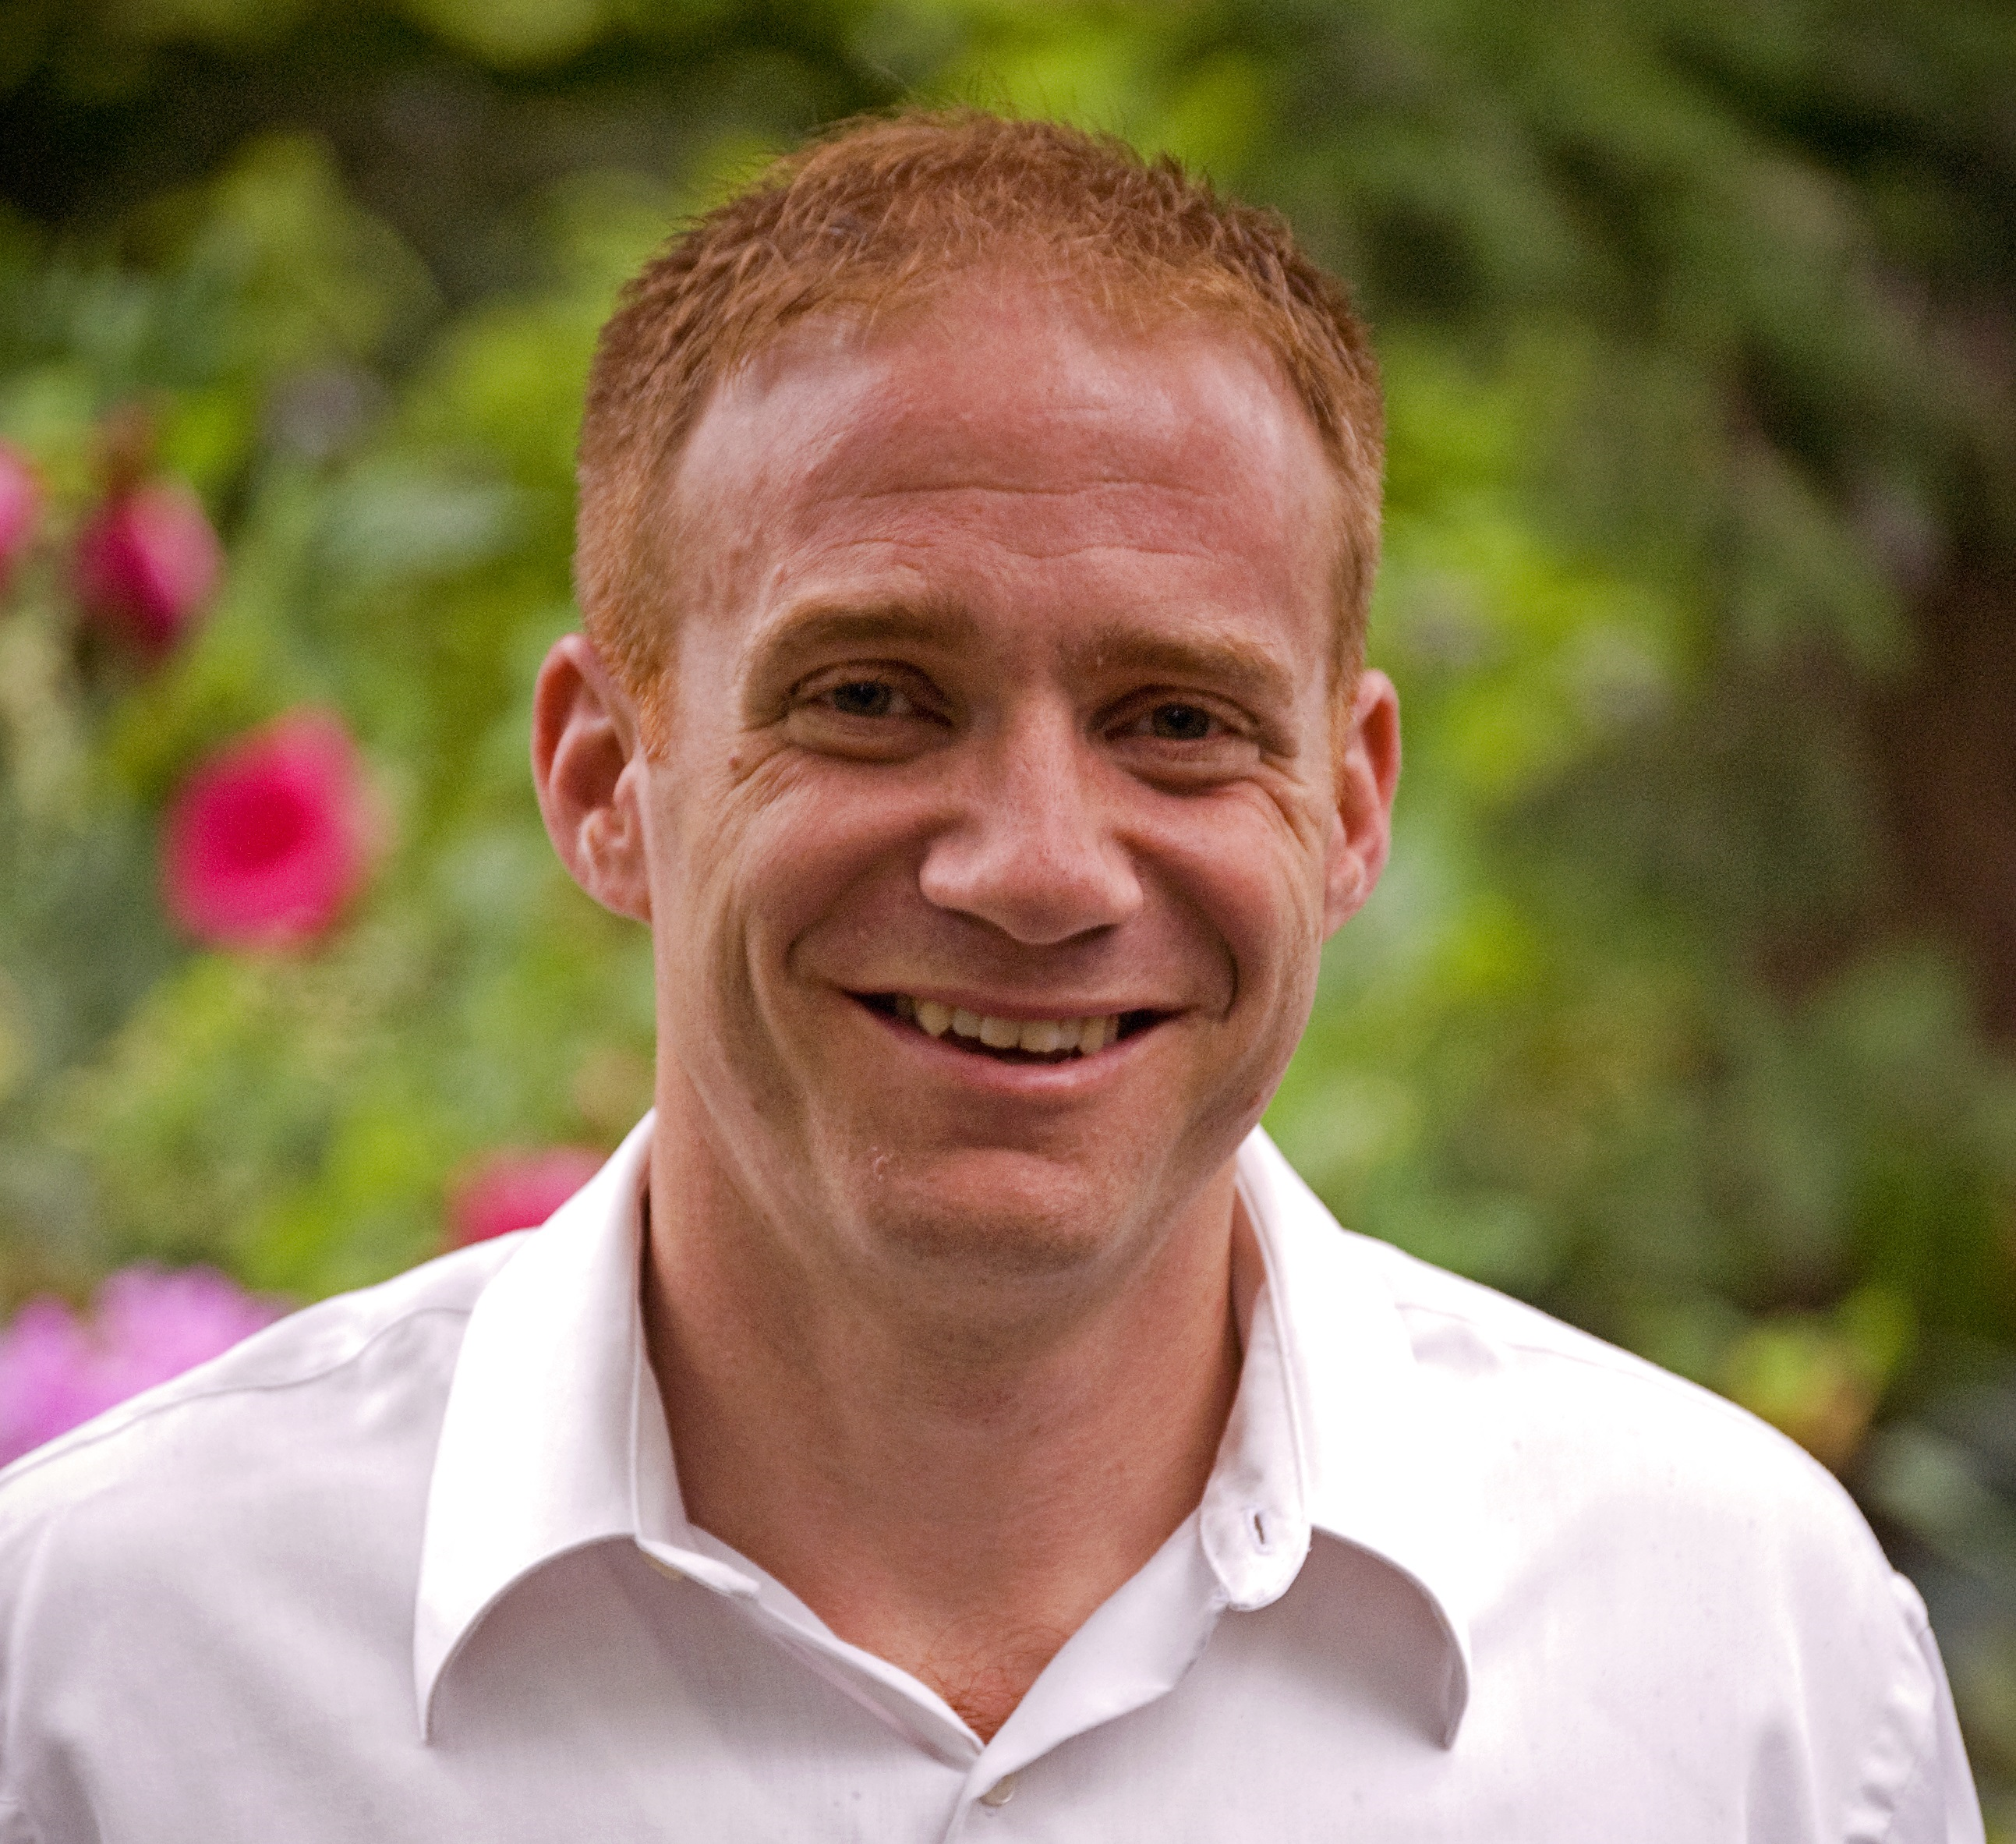
\includegraphics[width=1in,height=1.25in,clip,keepaspectratio]{figs/mw.jpg}}]{Michael Whalen}
Michael Whalen is the Director of the University of Minnesota Software Engineering Center and a consultant for Rockwell Collins, Inc.  Dr. Whalen is interested in formal analysis, language translation, testing, and requirements engineering.  He has developed simulation, translation, testing, and formal analysis tools for Model-Based Development languages including Simulink, Stateflow, and SCADE, and has published more than 60 papers on these topics.  He has led successful formal verification projects on large industrial avionics models, including displays (Rockwell-Collins ADGS-2100 Window Manager), redundancy management and control allocation (AFRL CerTA FCS program) and autoland (AFRL CerTA CPD program).  He has recently been researching tools and techniques for scalable compositional analysis, testing and system image generation from system architectural models for quadcopters and autonomous helicopters.
\end{IEEEbiography}

\begin{IEEEbiography}[{\includegraphics[width=1in,height=1.25in,clip,keepaspectratio]{figs/andrew.jpg}}]{Andrew Gacek}
Andrew Gacek is a Principal Industrial Logician in the Rockwell
Collins Advanced Technology Center. Andrew has a B.S. in Mathematics
and Computer Science from the University of Nebraska at Omaha, and
earned his M.S. and Ph.D. in Computer Science from the University of
Minnesota.

Andrew has an active interest in developing formal methods tools.  He
has built a variety of open-source and proprietary tools from static
analysis to model checking to theorem proving. His other interests
include formal logic, language translation, software design, operating
systems, and embedded systems.
\end{IEEEbiography}

\begin{IEEEbiography}[{\includegraphics[width=1in,height=1.25in,clip,keepaspectratio]{figs/mats.jpg}}]{Mats Heimdahl}
Mats Heimdahl is the Department Head and a Professor of Computer Science and Engineering at the University of Minnesota. He earned an M.S. in Computer Science and Engineering from the Royal Institute of Technology (KTH) in Stockholm, Sweden and a Ph.D. in Information and Computer Science from the University of California at Irvine.

His research interests are in software engineering, safety critical systems, software safety, testing, requirements engineering, formal specification languages, and automated analysis of specifications.

He is the recipient of the NSF CAREER award, a McKnight Land-Grant Professorship, the McKnight Presidential Fellow award, and the awards for Outstanding Contributions to Post-Baccalaureate, Graduate, and Professional Education at the University of Minnesota.
\end{IEEEbiography}

\end{document}
